% Options for packages loaded elsewhere
\PassOptionsToPackage{unicode}{hyperref}
\PassOptionsToPackage{hyphens}{url}
%
\documentclass[
]{article}
\usepackage{amsmath,amssymb}
\usepackage{lmodern}
\usepackage{iftex}
\ifPDFTeX
  \usepackage[T1]{fontenc}
  \usepackage[utf8]{inputenc}
  \usepackage{textcomp} % provide euro and other symbols
\else % if luatex or xetex
  \usepackage{unicode-math}
  \defaultfontfeatures{Scale=MatchLowercase}
  \defaultfontfeatures[\rmfamily]{Ligatures=TeX,Scale=1}
\fi
% Use upquote if available, for straight quotes in verbatim environments
\IfFileExists{upquote.sty}{\usepackage{upquote}}{}
\IfFileExists{microtype.sty}{% use microtype if available
  \usepackage[]{microtype}
  \UseMicrotypeSet[protrusion]{basicmath} % disable protrusion for tt fonts
}{}
\makeatletter
\@ifundefined{KOMAClassName}{% if non-KOMA class
  \IfFileExists{parskip.sty}{%
    \usepackage{parskip}
  }{% else
    \setlength{\parindent}{0pt}
    \setlength{\parskip}{6pt plus 2pt minus 1pt}}
}{% if KOMA class
  \KOMAoptions{parskip=half}}
\makeatother
\usepackage{xcolor}
\usepackage[margin=1in]{geometry}
\usepackage{graphicx}
\makeatletter
\def\maxwidth{\ifdim\Gin@nat@width>\linewidth\linewidth\else\Gin@nat@width\fi}
\def\maxheight{\ifdim\Gin@nat@height>\textheight\textheight\else\Gin@nat@height\fi}
\makeatother
% Scale images if necessary, so that they will not overflow the page
% margins by default, and it is still possible to overwrite the defaults
% using explicit options in \includegraphics[width, height, ...]{}
\setkeys{Gin}{width=\maxwidth,height=\maxheight,keepaspectratio}
% Set default figure placement to htbp
\makeatletter
\def\fps@figure{htbp}
\makeatother
\setlength{\emergencystretch}{3em} % prevent overfull lines
\providecommand{\tightlist}{%
  \setlength{\itemsep}{0pt}\setlength{\parskip}{0pt}}
\setcounter{secnumdepth}{-\maxdimen} % remove section numbering
\ifLuaTeX
  \usepackage{selnolig}  % disable illegal ligatures
\fi
\IfFileExists{bookmark.sty}{\usepackage{bookmark}}{\usepackage{hyperref}}
\IfFileExists{xurl.sty}{\usepackage{xurl}}{} % add URL line breaks if available
\urlstyle{same} % disable monospaced font for URLs
\hypersetup{
  hidelinks,
  pdfcreator={LaTeX via pandoc}}

\author{}
\date{\vspace{-2.5em}}

\begin{document}

\hypertarget{introduction}{%
\section{Introduction}\label{introduction}}

Statisticians use graphs in almost every stage of their work: we create
charts when we get new data, to explore what we have and identify
potential problems and opportunities. We fit models based on
relationships between variables which are often identified visually. We
identify problems with those models based on residual plots and other
visual diagnostics. When our modeling work has been completed, we
present our results to interested parties using visual displays, because
non-statisticians often find it easier to understand data and models
through an intuitive visual medium rather than through the mathematical
formulae which underlie the statistical work.

Given the wide range of uses for graphs and visual data displays in
statistical modeling, it is unsurprising that some graphs are more
useful for specific applications such as exploratory analysis, and are
unsuitable for other applications, such as presentation to an outside
group. In addition, we know that not all visual displays have equal
perceptual value {[}@aspillaga1996{]}. The best graphics are designed to
account for both the features of the dataset and the features of the
intended audience. Some design constraints stem from limitations of the
human perceptual system and are common to most potential consumers of
the visualization: the sine illusion {[}@vanderplas2015{]} affects
anyone with binocular depth perception, and color recommendations are
built around the specific characteristics of the human retina. Other
design constraints are due to the audience's experience level: are they
used to working with data? Do they understand specialized techniques
such as principal component analysis to the point where a plot of factor
loadings might be \svp{a} useful \svp{visual display}? When we create
visualizations for public consumption we have to consider both
perceptual factors and the target audience's domain knowledge. In this
introduction, we explore previous research related to the construction
of interactive and static visual displays for different audiences and
consider the implications of this research when designing interactive
data displays such as dashboards.

\svp{Most research in statistical graphics has been done on static graphics; usually, research also strips away all but the most essential contextual information. 
As a result, it can be hard to generalize this research to practical applications, where the contextual information surrounding the data is critical and the chart does not just exist in a vacuum.}

\svp{In the "real world", however, conventions and familiarity often win out over best practice validated by perceptual experiments.}

For example, in sports, many coaches desire printable diagrams
containing all necessary and valuable information on a single page. As
data in sports becomes more prominent, extensive, and collected, this
information must be refined.
\svp{Thus, in addition to the experimental evidence, we must consider the human element: how to introduce new graphical concepts to stakeholders, and the considerations involved in encouraging stakeholders to adopt these improved graphics.}
\svp{Let us first consider the audience characteristics that affect the selection of graphics. 
Then, we will engage with considerations based on the data to be displayed. 
Finally, we will consider the interactions between the audience and the data: how graphics are tested, amended, and hopefully eventually adopted into common use.}

\hypertarget{audience-considerations}{%
\subsection{Audience Considerations}\label{audience-considerations}}

Several factors, including perception, attention, and expertise, can
influence our desire and ability to read and engage with data
visualization.

\hypertarget{perception}{%
\subsubsection{Perception}\label{perception}}

\db{Why is it essential to comprehend perception laws when working with data visualization? 
First of all, they can guide your decision-making when creating a graph or dashboard. 
In addition, they assist the reader in quickly organizing and interpreting charts and graphs and making visual sense of the information.
Assigning meaning is not a statistical or computational step but a cognitive one. 
Each step in the data analysis process is part of a more extensive mental process.
To read reality from images is to solve a problem: a series of extremely difficult problems that persist throughout an individual's lifetime. 
Errors are illusions. 
Certain situations present unique challenges and lead to systematic errors; can these provide insight into how the brain solves the problem of which objects are represented by which images in general @gregory1968.
Human perception plays a direct role in the area of visualization and graphics. 
Data Analysis tasks closely resemble the cognitive process known as sensemaking. 
Tukey and Wilk highlight the role of cognitive processes in their initial descriptions of Exploratory Data Analysis (EDA) @tukey1966.
Additionally, short-term memory is crucial to the effectiveness of statistical graphics. 
Research indicates that our short-term memory can only store a limited amount of information at any given time. 
Therefore, designers must present data in a manner that is simple to comprehend and remember. 
Utilizing parallel coordinate plots is one method for achieving this. 
These plots enable viewers to compare multiple variables concurrently, thereby reducing cognitive load and making it easier to identify patterns and trends.}

\db{Untrained analysts can and do "analyze" data with only their natural mental abilities - The mind performs its data analysis-like process to create detailed understandings of reality from bits of sensory input.}

\db{The theory of Gestalt has philosophical and psychological roots that date back to the late 1800s. 
At its most basic, the entire form is perceived (or emerges to our visual pathways) as opposed to its component parts. 
Our visual interpretation of the world is a major factor in why humans perceive the world and its objects as organized, regular, and simple shapes, schemas, figures, or forms.
Without diving too deeply into sensory perception, brain pathways, and the biology of the eye, let's establish two essential facts:}

\begin{enumerate}
\def\labelenumi{(\arabic{enumi})}
\item
  Vision, and how we perceive or interpret what we see, is primarily the
  result of our brain and nervous system transmitting sensory stimuli
  through neural pathways. This is why people with perfectly functioning
  eyes, such as those with Cortical Visual Impairment, may be unable to
  see if the pathways to the brain are miswired or damaged (see a viz on
  that here).
\item
  While 70\% of our experience of the world is gained through vision,
  our brains can only simultaneously process less than 5\% of our visual
  environment.
\end{enumerate}

\db{All of this suggests that our brain frequently perceives things differently than what is actually present. 
If you are familiar with optical illusions or the famous "gorilla in the crowd" experiment, you are aware that we do not always process everything in our visual field. 
There is simply too much information for our brains to process, and if we tried to interpret it all, we would be rendered paralyzed.
We organize the world according to Gestalt principles and pre-attentive attributes so that it is familiar, makes sense, and is easy to process.
These principles guide how people perceive and make sense of the world around them, and they play a critical role in designing effective visual displays, such as dashboards.}

Gestalt principles include:

\begin{itemize}
\tightlist
\item
  Proximity: Objects close to each other are perceived as related or
  grouped.
\item
  Similarity: Objects that are similar in some way (e.g., shape, color,
  size) are perceived as related or grouped.
\item
  Continuation: The human eye follows lines and patterns, so designers
  can use this principle to guide the viewer's gaze through a display.
\item
  Closure: The human brain tends to complete incomplete figures or
  patterns, so designers can use this principle to create the illusion
  of missing information.
\item
  Figure-Ground: The human brain separates the foreground (figure) from
  the background (ground), so designers can use this principle to create
  visual hierarchy and emphasis.
\item
  Contrast: The human eye is drawn to high-contrast areas, so designers
  can use this principle to create emphasis and hierarchy.
\item
  Symmetry and Balance: The human eye finds symmetry and balance
  visually pleasing, so designers can use this principle to create a
  sense of harmony and order.
\end{itemize}

\begin{figure}

{\centering 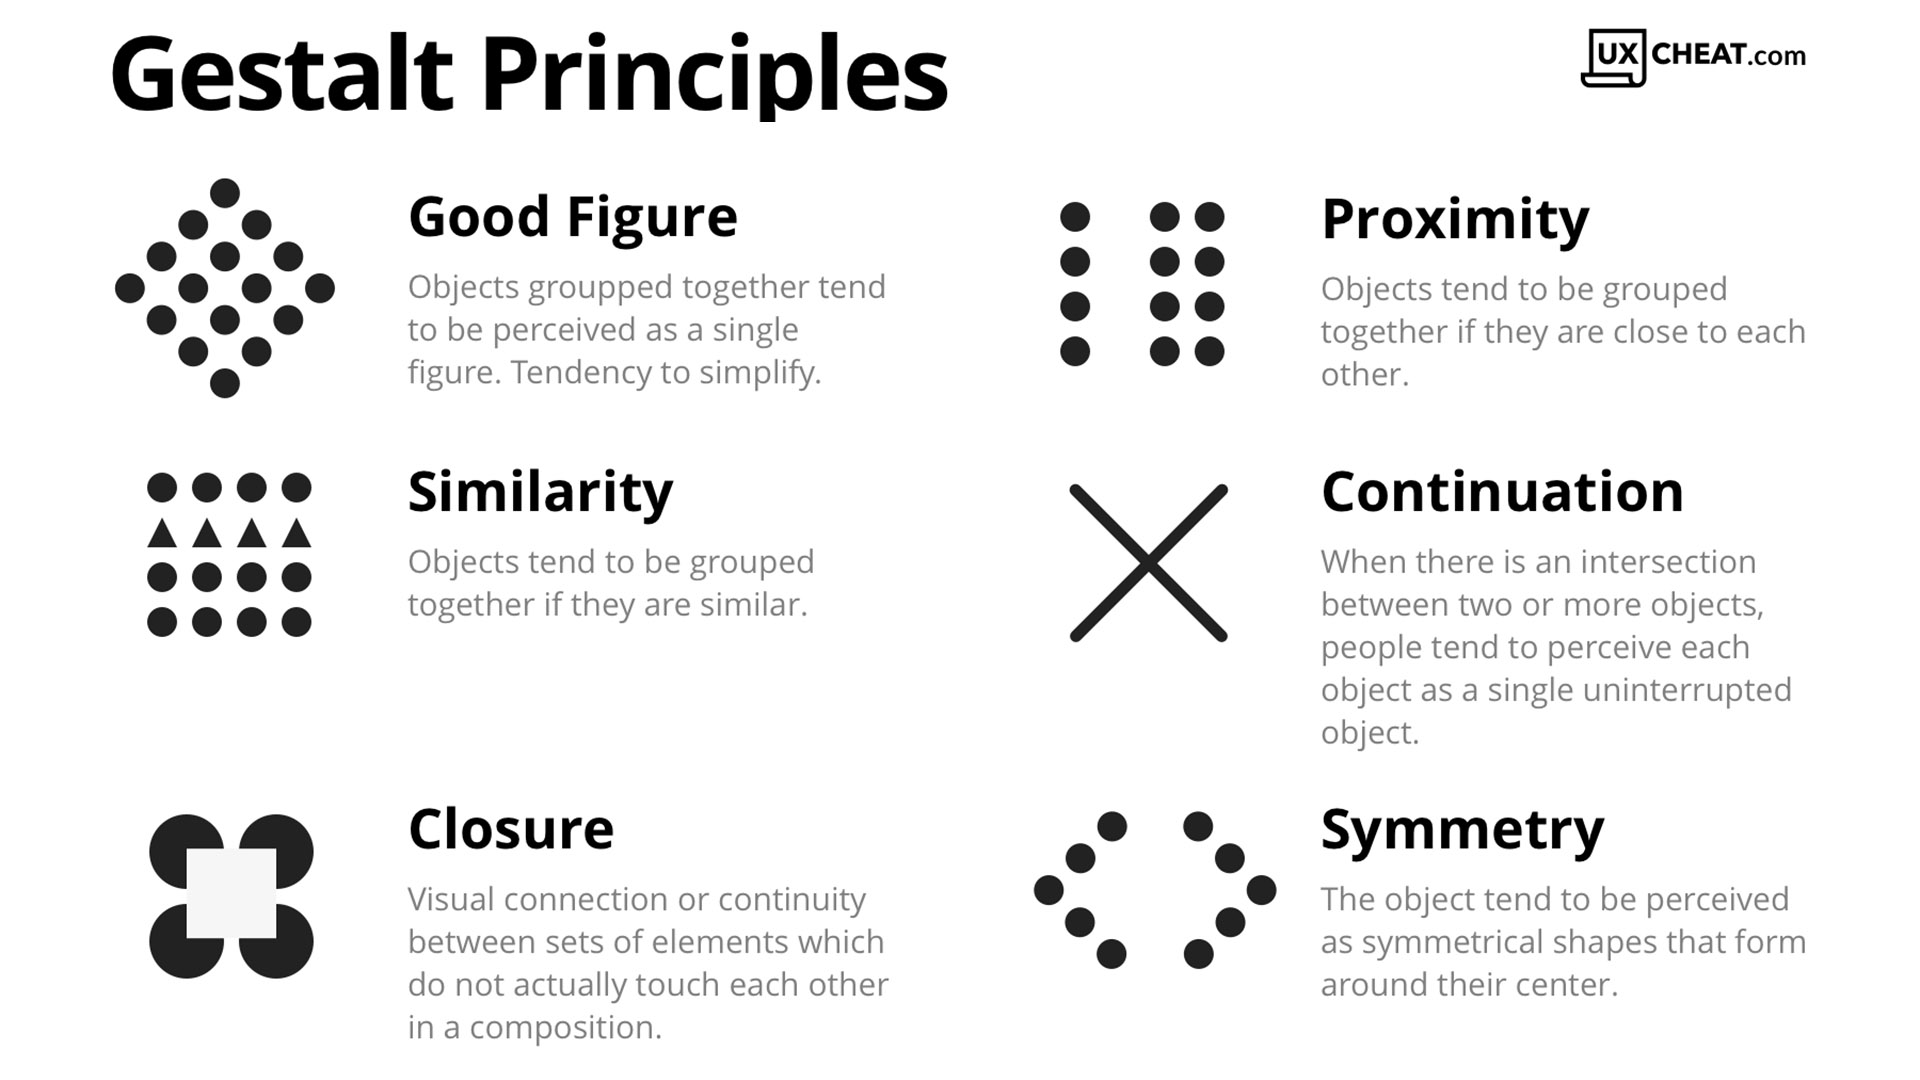
\includegraphics[width=0.75\linewidth]{figure/gestalt_principles} 

}

\caption{Gestalt Principles with Examples}\label{fig:gestalt}
\end{figure}

\db{These principles are based on cognitive psychology and understanding how the human brain processes visual information.}

\db{Eye tracking regression is a method used in eye tracking studies to analyze eye movement data and identify the factors that influence a participant's gaze behavior. 
In eye tracking regression, the eye movement data is regressed on a set of predictor variables, such as visual features of the stimulus or task instructions, to determine the degree of influence each variable has on eye movements.
On the other hand, statistical regression is a technique used in statistics to identify the relationship between a dependent variable and one or more independent variables. 
Statistical regression is used to make predictions or to explain the relationship between variables. 
It is used in various fields, such as economics, psychology, and biology, to analyze and understand complex data.
While both techniques involve regression analysis, they are used for different purposes and with different types of data. 
Eye-tracking regression is specific to eye-tracking data and is used to understand visual attention and perception. 
Statistical regression, however, is a more general technique that can be applied to any type of data and is used for modeling relationships between variables.}

\hypertarget{attention-and-memory}{%
\subsubsection{Attention and Memory}\label{attention-and-memory}}

Short-term memory (STM), also known as working memory, is the stage of
temporary storage and processing where the majority of memory retention
effort is expended. According to @baddeley2012, STM is a
limited-capacity system prone to interference and decay. Selective
attention is essential for the maintenance of STM because it allows us
to filter out irrelevant information and concentrate on what is
essential @cowan2001.

Visual aids such as charts and diagrams can improve short-term memory by
allowing us to encode and retain information more effectively, according
to research @alvarez2004.

Consequently, utilizing visual aids such as charts can be advantageous
for enhancing our short-term memory.

Furthermore, annotations can also be useful in aiding short-term memory.
By adding annotations, such as notes or highlights, to information we
are trying to remember, we can improve our recall of the information
later on @alvarez.

According to the Feature Integration Theory (FIT), STM is composed of
two stages: pre-attentive processing and focused attention
@treisman1998. Parallel and independently, the brain processes the
physical characteristics of an object, such as its color, shape, and
orientation, during pre-attentive processing. However, focused attention
is required to bind these features into a coherent object representation
in STM. STM can be improved through various strategies, such as
rehearsal, chunking, and elaboration @oberauer2009. For example, by
repeating a phone number several times or breaking it down into chunks
of two or three digits, we can increase the likelihood of it being
stored in STM. Similarly, by elaborating on the information we want to
remember, such as creating mental associations or visual images, we can
enhance its retention in STM @bui2015.

STM is a dynamic and malleable cognitive system that is crucial to our
daily lives. Understanding the mechanisms underlying STM and how to
improve it can have significant implications for learning, memory, and
the treatment of memory disorders.

\hypertarget{constructing-meaning}{%
\subsubsection{Constructing Meaning}\label{constructing-meaning}}

Gestalt psychology suggests that humans actively construct meaning by
organizing information into patterns and wholes @wertheimer1923. Both
top-down and bottom-up processing are involved in the process of meaning
construction. Bottom-up processing entails analyzing sensory data from
the environment and constructing perceptions based on this data.
Top-down processing is the influence of prior knowledge, expectations,
and context on the perception and interpretation of incoming sensory
data.

Together, top-down and bottom-up processing facilitate the encoding and
retrieval of information in the context of short-term memory. Selective
attention, the ability to focus on relevant information while ignoring
irrelevant information, is an example of top-down processing that aids
in the encoding and retrieval of information in short-term memory
@cowan2010.\\
According to the feature integration theory, the perception of objects
involves both the bottom-up analysis of individual features and the
top-down processing of higher-level features in order to form a complete
perception @treisman1980.

The Gestalt principles of perception emphasize the significance of
bottom-up and top-down processing in constructing meaning from sensory
data. Both types of processing are involved in encoding and retrieving
information, which has significant implications for understanding how
short-term memory works.

\hypertarget{expertise}{%
\subsubsection{Expertise}\label{expertise}}

The development of expertise is a gradual and iterative process that is
influenced by numerous psychological factors, such as cognitive
processes, automaticity, readily accessible information, and practice
effects.

Cognitive Processes - the way we think about and approach a task.

As we become more proficient in a particular skill, we develop more
complex and efficient mental models or schemata. These mental models
help us to organize information in a meaningful way, and to quickly
identify and solve problems related to the task. This process is known
as cognitive restructuring and is facilitated by developing
domain-specific knowledge @ericsson1996. For example, a chess master is
able to quickly recognize patterns and positions on the board that are
common in chess, which allows them to make decisions more quickly and
accurately than a novice player.

Automaticity - the ability to perform a task without conscious effort or
attention

As our proficiency in a task increases, our performance becomes more
automatic, thereby freeing up cognitive resources for other tasks. The
development of procedural knowledge, which is the ability to perform a
series of steps or actions in a particular order, facilitates this
process @Fitts1967. For instance, a skilled typist can type without
looking at the keyboard because their finger movements have become
automatic.

Information Readily Available - the way we process information related
to a task

As our proficiency increases, we can recognize and retrieve pertinent
information more rapidly and precisely than a novice. This is made
possible by the creation of domain-specific knowledge structures that
allow us to retrieve pertinent information from memory quickly
@Chase1973. For instance, a medical expert can quickly identify signs
and diagnose a patient using their knowledge of disease symptoms and
risk factors.

Practice Effects - extensive practice and experience

Practice effects are the performance enhancements that result from
repeated practice. These gains are frequently most significant at the
outset of practice, but gradually diminish as the individual approaches
their performance ceiling @Anderson1982. The development of procedural
knowledge and automaticity, which allow for more efficient and accurate
task performance, facilitates the effects of the practice.

\hypertarget{engagement-with-the-data}{%
\subsubsection{Engagement with the
data}\label{engagement-with-the-data}}

\db{<!-- This is a good paragraph -- but I'm not sure it's in the right place.  -->
The goal of data analysis is to extract meaningful insights, patterns, and knowledge from data. 
The process of data analysis involves collecting, cleaning, transforming, and modeling data, followed by the use of statistical and machine learning methods to uncover patterns and relationships within the data. 
The end goal of data analysis is to support decision making and provide a basis for informed action. 
Data analysis can help organizations to better understand their customers, market trends, and operational performance. 
<!-- What about organizations which aren't profit-driven? They still need to understand the relationship between different variables in the dataset. -->
Additionally, data analysis can support scientific research by helping researchers to test hypotheses, develop theories, and gain a deeper understanding of complex phenomena. 
Ultimately, data analysis aims to turn data into actionable insights and information that can inform and improve decision-making.}

\db{Visualizing Complex Data is representing complex, multi-dimensional data in a graphical or pictorial form to make it easier to understand and interpret. 
The goal is to turn large, intricate data sets into visually appealing and intuitive representations, such as charts, graphs, maps, and other types of visualizations, to help identify patterns, trends, and relationships that may not be immediately apparent from raw data. 
This process can help to communicate complex information effectively and make data-driven decisions.}

William Cleveland's subcycle plots:

\begin{itemize}
\tightlist
\item
  glyph maps and binned graphics emerging from big data visualization
  efforts.
\item
  glyphs and other plots have been embedded in maps
\end{itemize}

Bertin's Semiologic of Graphics is a seminal work in the academic study
of visualization. Glyphmaps have been developed as a tool for tracking
climate and climate change data {[}@wickham2012{]}; {[}@hobbs2010{]}.
{[}@schulz2013{]} define two abstractions for the design of
visualizations:

\begin{center}
\begin{align*}
  Data + Task = Visualization \\
  Data + Visualization = Task
\end{align*}
\end{center}

\db{These abstractions demonstrate dependence between the data, visual representation, and the task. 
The more the user interacts with the visualization, they gain knowledge. 
The interactions allow the user to control their understanding by providing the flexibility to create new views that help them go beyond just the visual representation [@kiem2008]. 
The field of information visualization is continually adapting to changes with the big data revolution.}

\db{Data Scientists and Statisticians have produced more graphics since the pandemic's start. 
The reasons someone will create a graphic or dashboard may include but are not limited to understanding raw data structures to analyze model assumptions and present predictions, along with displaying key performance metrics of business logic. 
These goals help work to navigate and are best served by quick-and-dirty representations of the data, while highly polished graphics may be more useful in other situations. 
It is valuable and essential to convey data correctly, meaning that we need to understand how graphics are perceived on a dashboard on a general level. Previous research by Tukey focused on graphics as a tool for exploratory analysis. 
Tukey describes in Exploratory Data Analysis [@tukey1966] that pictures are often used to display data in a more enhanced version than a table. 
Tukey outlines detailed the types of different graphics and in which situations to utilize these graphics. 
The article - "External cognition: how do graphical representations work?" by Scaife and Rogers [@scaife1996] critique the disparate literature on graphical representations, focusing on four representative studies. 
In general, this will help in the psychology of the perceptual experience.}

\db{The visual reference model developed by Card et al. [@Card] describes and identifies the three phases of the visualization process.}

\begin{figure}

{\centering 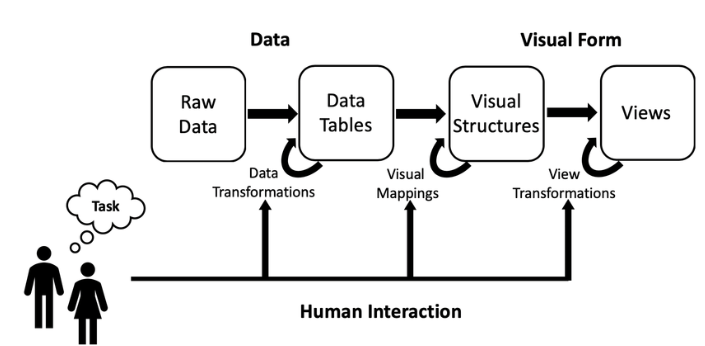
\includegraphics[width=0.75\linewidth]{figure/VizModelDiagram} 

}

\caption{Visual Reference model by Card}\label{fig:graphics}
\end{figure}

\db{While External Cognition describes the advances in graphical technology and how little had been done in the work of the cognitive framework of the discipline, the following citations by Ware attempt to develop the necessary guidelines that are useful for the work done by the perceptual experience.}

Colin Ware ``Information Visualization: Perception for Design''
{[}@Ware2004{]} there are four stages of visualization

\begin{itemize}
\tightlist
\item
  The collection and storage of data itself
\item
  The preprocessing design to transform the data into something we can
  understand
\item
  The display hardware and the graphics algorithms produce the image on
  the screen.
\item
  The human perceptual and cognitive system
\end{itemize}

\db{The overlapping understanding in the field, while Ware takes the process one step further not just to allow the end user to understand the outcomes but to curate the outcomes with a visual perception of the data that makes the cognitive load easier for the end-user.}

\db{A dashboard has much information related to tabular data from multiple sources. 
Design should be recorded a produced with content that will allow for reproducibility. 
A dashboard should have some content related to interaction with the user. 
This interaction can be in multiple forms: toggling through the selection of variables to display uniformly to the use of interaction on the graph and allowing a user to understand best what is being shown in the diagram.}

\db{The entire dashboard/Interface should have a human perception piece that is useful for the user to comprehend and use. 
For example, the dashboard/interface could be more practical if the user is visually overwhelmed.}

\begin{itemize}
\tightlist
\item
  Identified the highly relevant from a dashboard design perspective
  {[}@odonnell2000{]}
\end{itemize}

\begin{enumerate}
\def\labelenumi{\arabic{enumi}.}
\tightlist
\item
  Information systems give interaction and feedback
\item
  Type of presentation format to be used
\item
  Differences in the amount of information load.
\end{enumerate}

Information load is essential, as dashboards must provide the right
decision cues without overwhelming the user with excess information.

\db{"A decision cue is a feature of something perceived that is used in the interpretation of perception" [@choo2009],  where perception is an inferential process as objects in the environment can only be perceived indirectly through available information that has been sensed by the individual [@brunswik1952].}

\db{Visual complexity and information utility are required. 
Visual complexity refers to the "degree of difficulty in providing a verbal description of an image ([@heaps1999], [@olivia2004]).}

\begin{itemize}
\tightlist
\item
  Graphs are more suitable for spatial tasks (ex., for comparing a set
  of values) {[}@vessey1991{]};{[}@umanath1994{]};{[}@vessey1994{]}
\item
  Graphs reduced the negative influence of information overload
\item
  Graphs produced better correlation estimates and decreased time on a
  task {[}@schulzand{]};{[}@booth2006{]}
\item
  Self-organizing maps and multidimensional scaling did not
  significantly outperform tabular representations {[}@huang2006{]}
\end{itemize}

The purposes of a dashboard:

\begin{enumerate}
\def\labelenumi{\arabic{enumi}.}
\tightlist
\item
  Consistency
\item
  Monitoring
\item
  Planning
\item
  Communication
\end{enumerate}

\db{Card stated "Use interactive visual representations of abstract, non-physically based data to amplify cognition." [@card1999]}

\db{Visual perception involves two elements - the perceptual and conceptual gist. 
The perceptual gist refers to the process of the brain when it determines the image properties that provide the structural representation of a scene, like color and texture. 
The conceptual gist refers to the scene's meaning, which is improved after the perceptual information is received ([@friedman1979]; [@olivia2004]).}

\db{Visual complexity might increase with the quality and range of objects and with varying material and surface styles [@heylighen1997].}

\db{Repetitive and uniform patterns and existing knowledge of the objects in the scene reduce visual complexity [@olivia2004].}

\db{If the guidelines on our visual information load can be related to statistical terminology, we can consider this the fisher information of visual information load. 
This load can be used as a metric for balancing the amount of information rather than overloading the consumer.}

Visual Data Mining

\db{For data mining to be effective, it is important to include humans in the data exploration process and combine the flexibility, creativity, and general knowledge of the computational power of today's computers. 
Visual data exploration aims at integrating humans in the data exploration process, applying their perceptual abilities to the large data sets available in today's computer systems [@kiem2002].}

The visual data exploration process can be seen as a hypothesis
generation process:

\begin{itemize}
\tightlist
\item
  The visualizations of the data allow the user to gain insight into the
  data and come up with new hypotheses
\item
  Along with verification of the hypotheses
\end{itemize}

The main advantages of visual data exploration over automatic data
mining techniques from statistics or machine learning are:

\begin{itemize}
\tightlist
\item
  visual data exploration can efficiently deal with highly inhomogeneous
  and noisy data.
\item
  visual data exploration is intuitive and requires no understanding of
  complex mathematical or statistical algorithms or parameters.
\end{itemize}

\db{Visual Exploration Paradigm, also known as MGV (Massive Graph Visualizer), is an integrated visualization and exploration system for massive multidigraph navigation [@abello2002]. 
MGV usually follows a three-step process:}

\begin{itemize}
\tightlist
\item
  overview first
\item
  zoom and filter
\item
  details-on-demand
\end{itemize}

\db{The user identifies interesting patterns and focuses on one or more of them. Note that visualization technology does not only provide the base visualization techniques for all three steps but also bridges the gap between the steps.}

Visualization Technique Classification:

\begin{itemize}
\tightlist
\item
  Standard 2D/3D displays such as bar charts and x-y plots
\item
  Geometrically transformed displays, such as landscapes and parallel
  coordinates, as used in a scalable framework
\item
  Icon-based displays such as needle icons and star icons as used in MGV
\item
  Dense pixel displays such as the recursive pattern and circle segments
  techniques and the graph sketches as used in MGV
\item
  Stacked displays, such as treemaps or dimensional stacking
\end{itemize}

Interaction and distortion techniques allow users to interact directly
with the visualizations.

\begin{itemize}
\tightlist
\item
  Projection as used in the Grand Tour System
\item
  Filtering as used in Polaris
\item
  Zooming as used in MGV and scalable framework
\item
  Linking and Brushing as used in Polaris and the scalable framework
\end{itemize}

Design Theory in Information System

The knowledge is distinguished as the fifth of five types of theory:

\begin{enumerate}
\def\labelenumi{\arabic{enumi}.}
\tightlist
\item
  Analyzing \& describing
\item
  Understanding
\item
  Predicting
\item
  Explaining and predicting
\item
  Design and action
\end{enumerate}

\db{A definition of information systems that are suitable for our purposes concerns: "the effective design delivery use and impact of information technology in organizations and society [@avison1995]. }

The two paradigms characterize much of the research in the Information
systems discipline:

\begin{itemize}
\tightlist
\item
  \emph{Behavioral Science Paradigm} - seeks to develop and verify
  theories that explain or predict human or organizational behavior
  (roots in natural science research methods).
\item
  \emph{Data Science Paradigm} - seeks to extend the boundaries of human
  and organizational capabilities by creating new and innovative
  artifacts (roots in engineering and the sciences of the artificial)
  {[}@simon1996{]}.
\end{itemize}

\db{Technology and behavior are not dichotomous in an information system. They are inseparable [@lee2000]. Information technology (IT) artifacts are broadly defined as:}

\begin{itemize}
\tightlist
\item
  constructs (vocabulary \& symbols)
\item
  models (abstractions \& representations)
\item
  methods (algorithms \& practices)
\item
  instantiations (implemented \& prototype systems)
\end{itemize}

\db{These are concrete prescriptions that enable IT researchers and practitioners to understand and address the problems inherent in developing and successfully implementing information systems within organizations ([@march1995]; [@nunamaker1991]). }

\hypertarget{data-considerations}{%
\subsection{Data Considerations}\label{data-considerations}}

\db{Exploratory Data Analysis (EDA) analyzes and summarizes a dataset to discover patterns, trends, and insights. 
It is a crucial step in the data analysis process and is often used to identify which variables are essential, what the data looks like, and what the underlying structure of the data is. 
EDA is typically done using various techniques, such as visualizations, statistical summaries, and data transformations.}

\db{John Tukey was the first to organize the collection and methods associated with philosophy into Exploratory Data Analysis (EDA). 
John Tukey, creator of stem-and-leaf plot, boxplot-resistant smooth, and the violin plot (also known as rootgram) who taught us to utilize these methods to organize and demonstrate EDA. 
He was a strong advocate for the importance of EDA as a crucial first step in the data analysis process and emphasized the need for visualization and interactive techniques to understand patterns and relationships in data.}

\begin{center}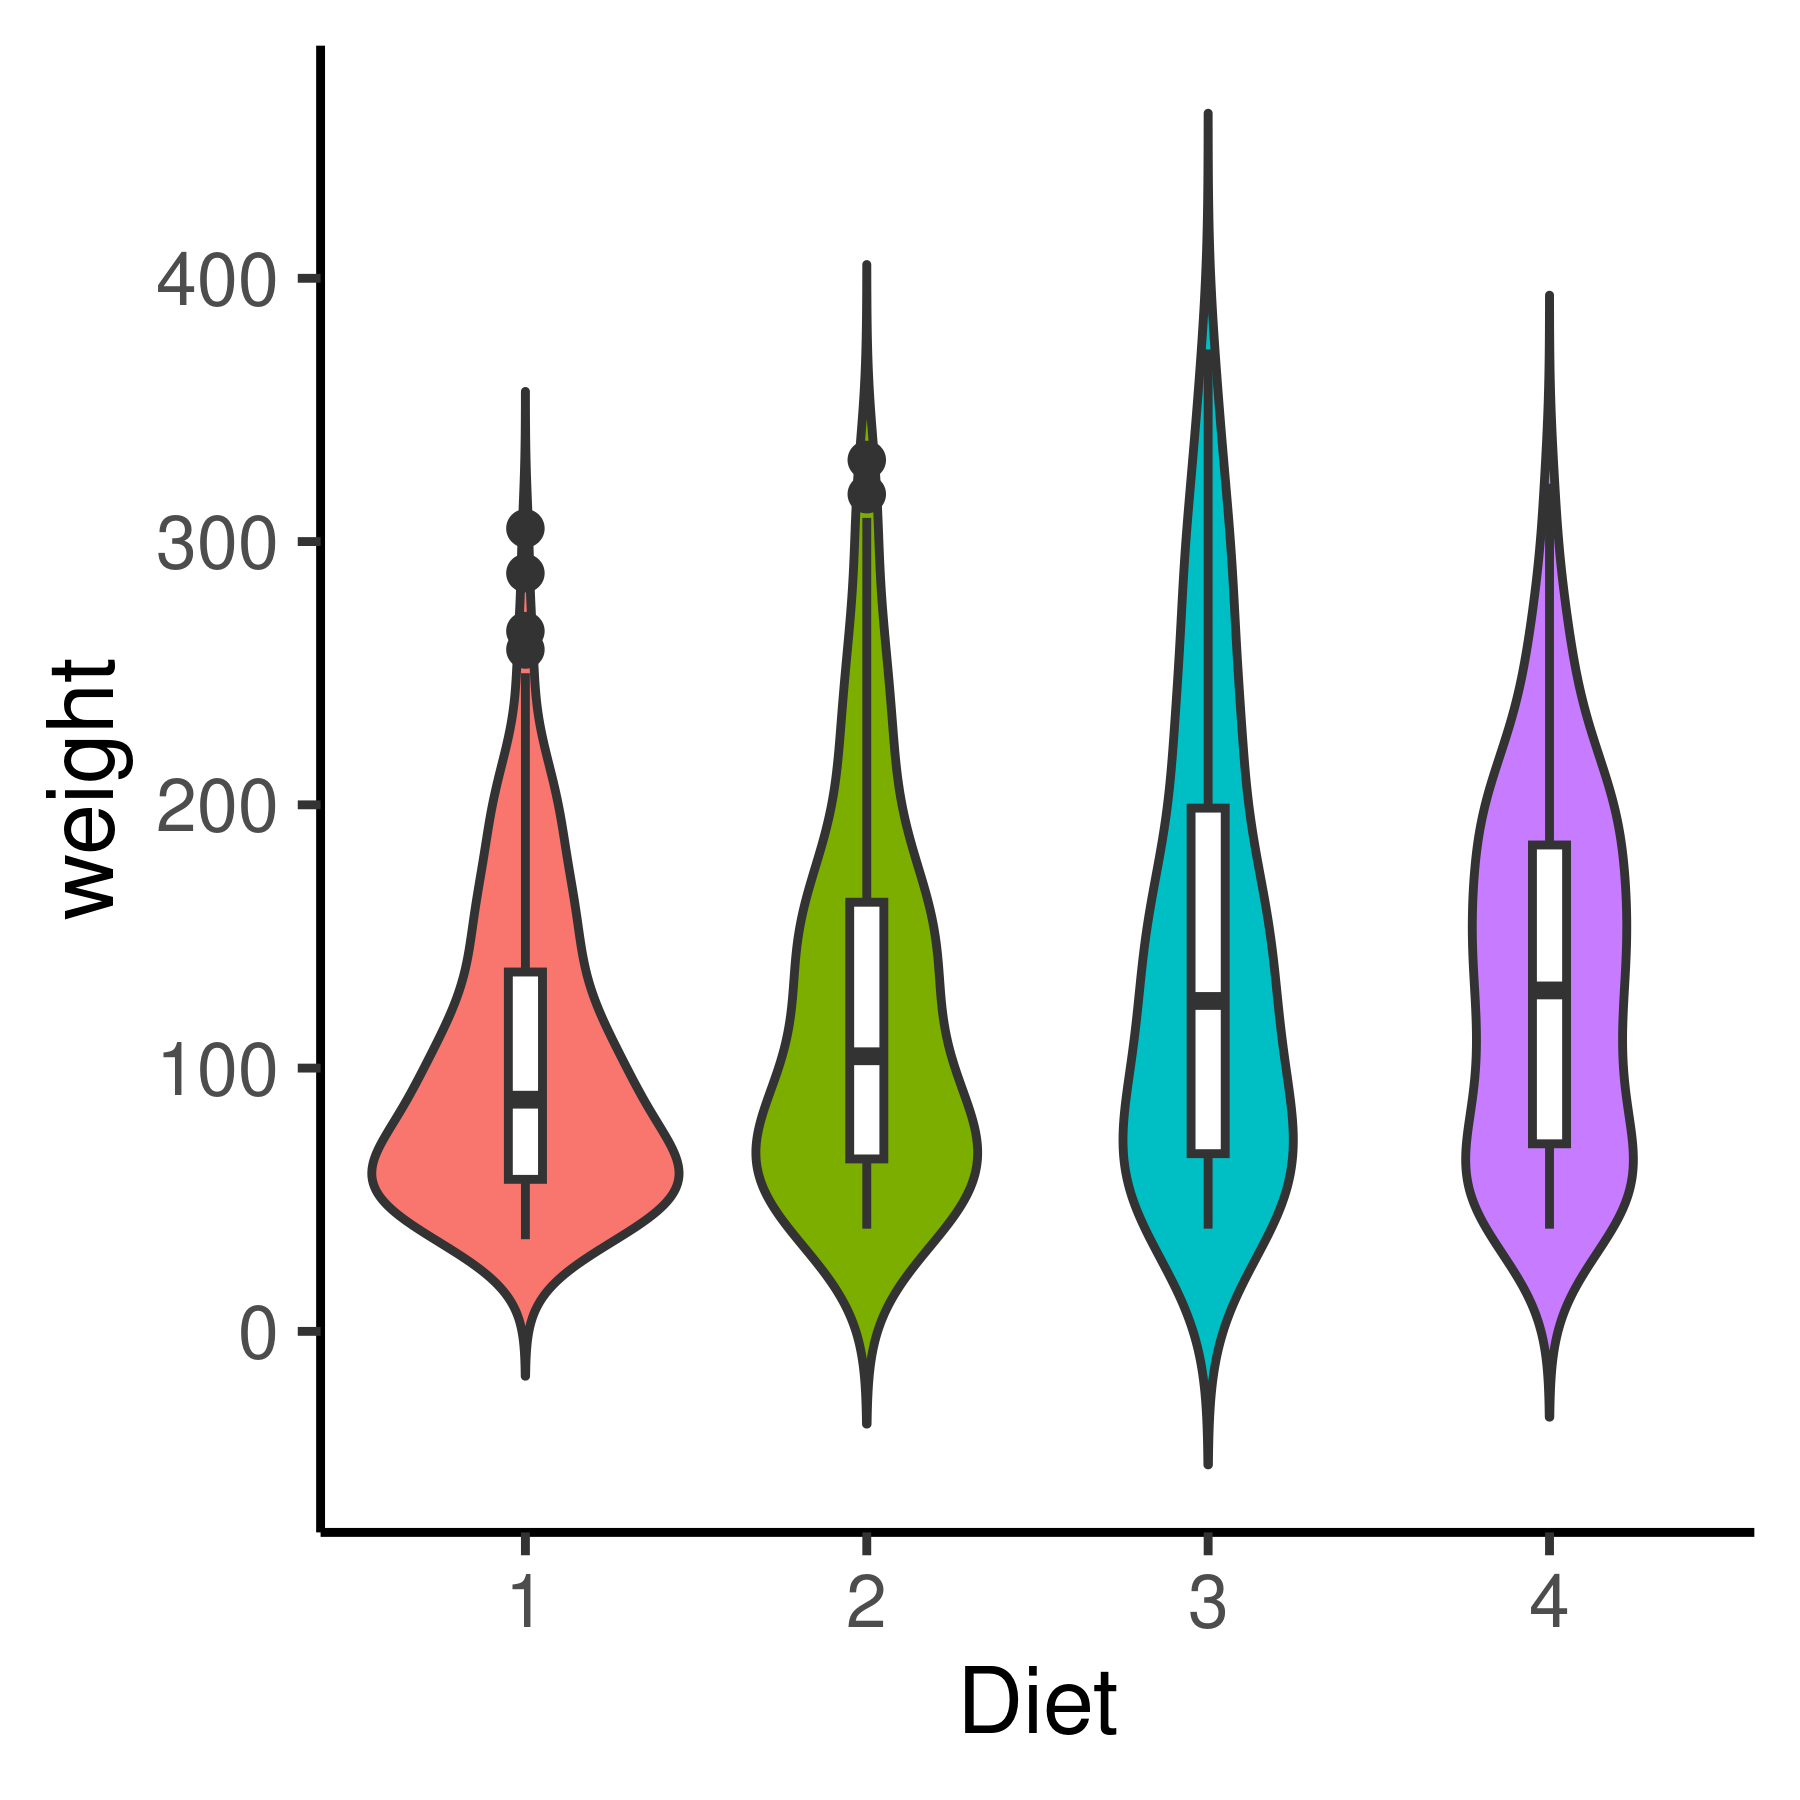
\includegraphics[width=.49\linewidth]{01-lit-review_files/figure-latex/violin_plot-1} 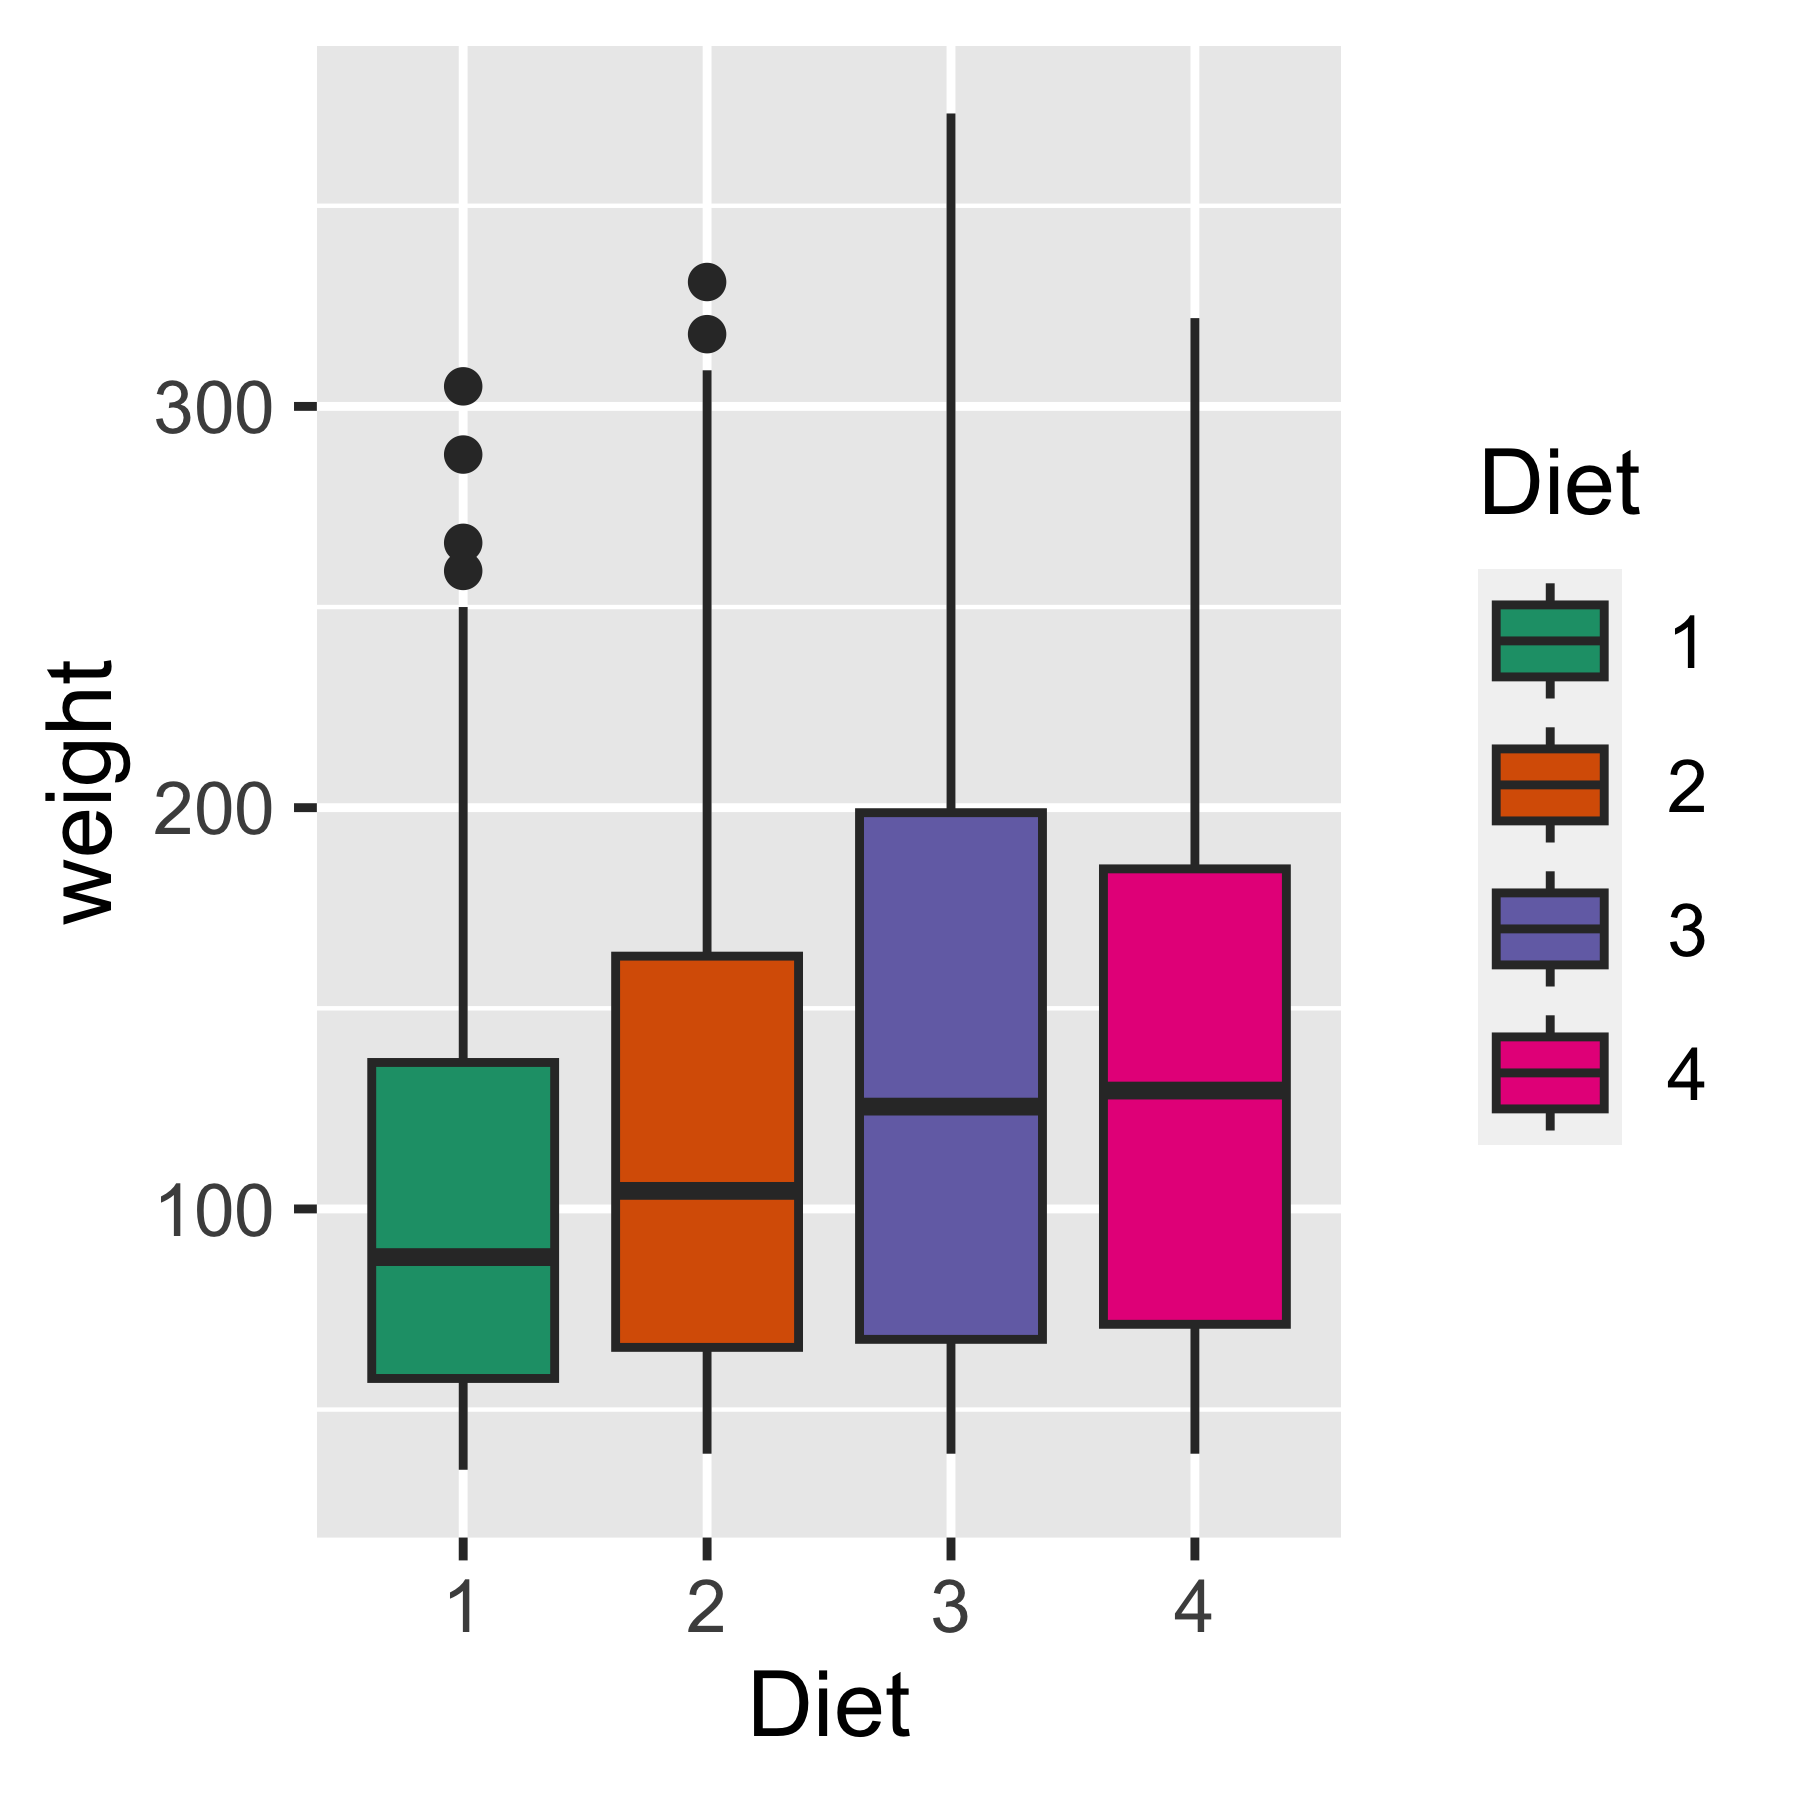
\includegraphics[width=.49\linewidth]{01-lit-review_files/figure-latex/violin_plot-2} \end{center}

\db{Tukey's Principles in EDA:}

\begin{enumerate}
\def\labelenumi{\arabic{enumi}.}
\tightlist
\item
  Graphical exploration looking for patterns or displaying fit.
\end{enumerate}

\begin{itemize}
\tightlist
\item
  The method demonstrates things about data that are not understood by a
  single numeric metric. This has been useful in graphing the data
  before you develop summary statistics.
\end{itemize}

\begin{enumerate}
\def\labelenumi{\arabic{enumi}.}
\setcounter{enumi}{1}
\tightlist
\item
  Describing the general patterns of the data.
\end{enumerate}

\begin{itemize}
\tightlist
\item
  This step should be insensitive to outliers. In general, think about
  the types of resistant measures (i.e., median or mean). This step is
  making sure to determine data patterns.
\end{itemize}

\begin{enumerate}
\def\labelenumi{\arabic{enumi}.}
\setcounter{enumi}{2}
\item
  The natural scale/state that the data are at their best. This will be
  the step at which the scale of data can be helpful for analysis. The
  reexpressing data to a new scale by taking the square root or
  logarithmic scale.
\item
  The mostly known parts of EDA but is done in the way of accessing fit
  of the data. This is taught in every statistics 101 class. The growth
  of machine learning and prediction methods have now used residuals
  more in the toolbox to assessing the best prediction models.
\end{enumerate}

\begin{itemize}
\tightlist
\item
  The idea generally is to determine the deviations in the data from a
  general pattern by looking at the data from the fit of the data.\}
\end{itemize}

\begin{verbatim}
## Warning: Groups with fewer than two data points have been dropped.
\end{verbatim}

\begin{verbatim}
## Warning: Removed 1 rows containing missing values (`position_stack()`).
\end{verbatim}

\begin{verbatim}
## `stat_bin()` using `bins = 30`. Pick better value with `binwidth`.
\end{verbatim}

\begin{center}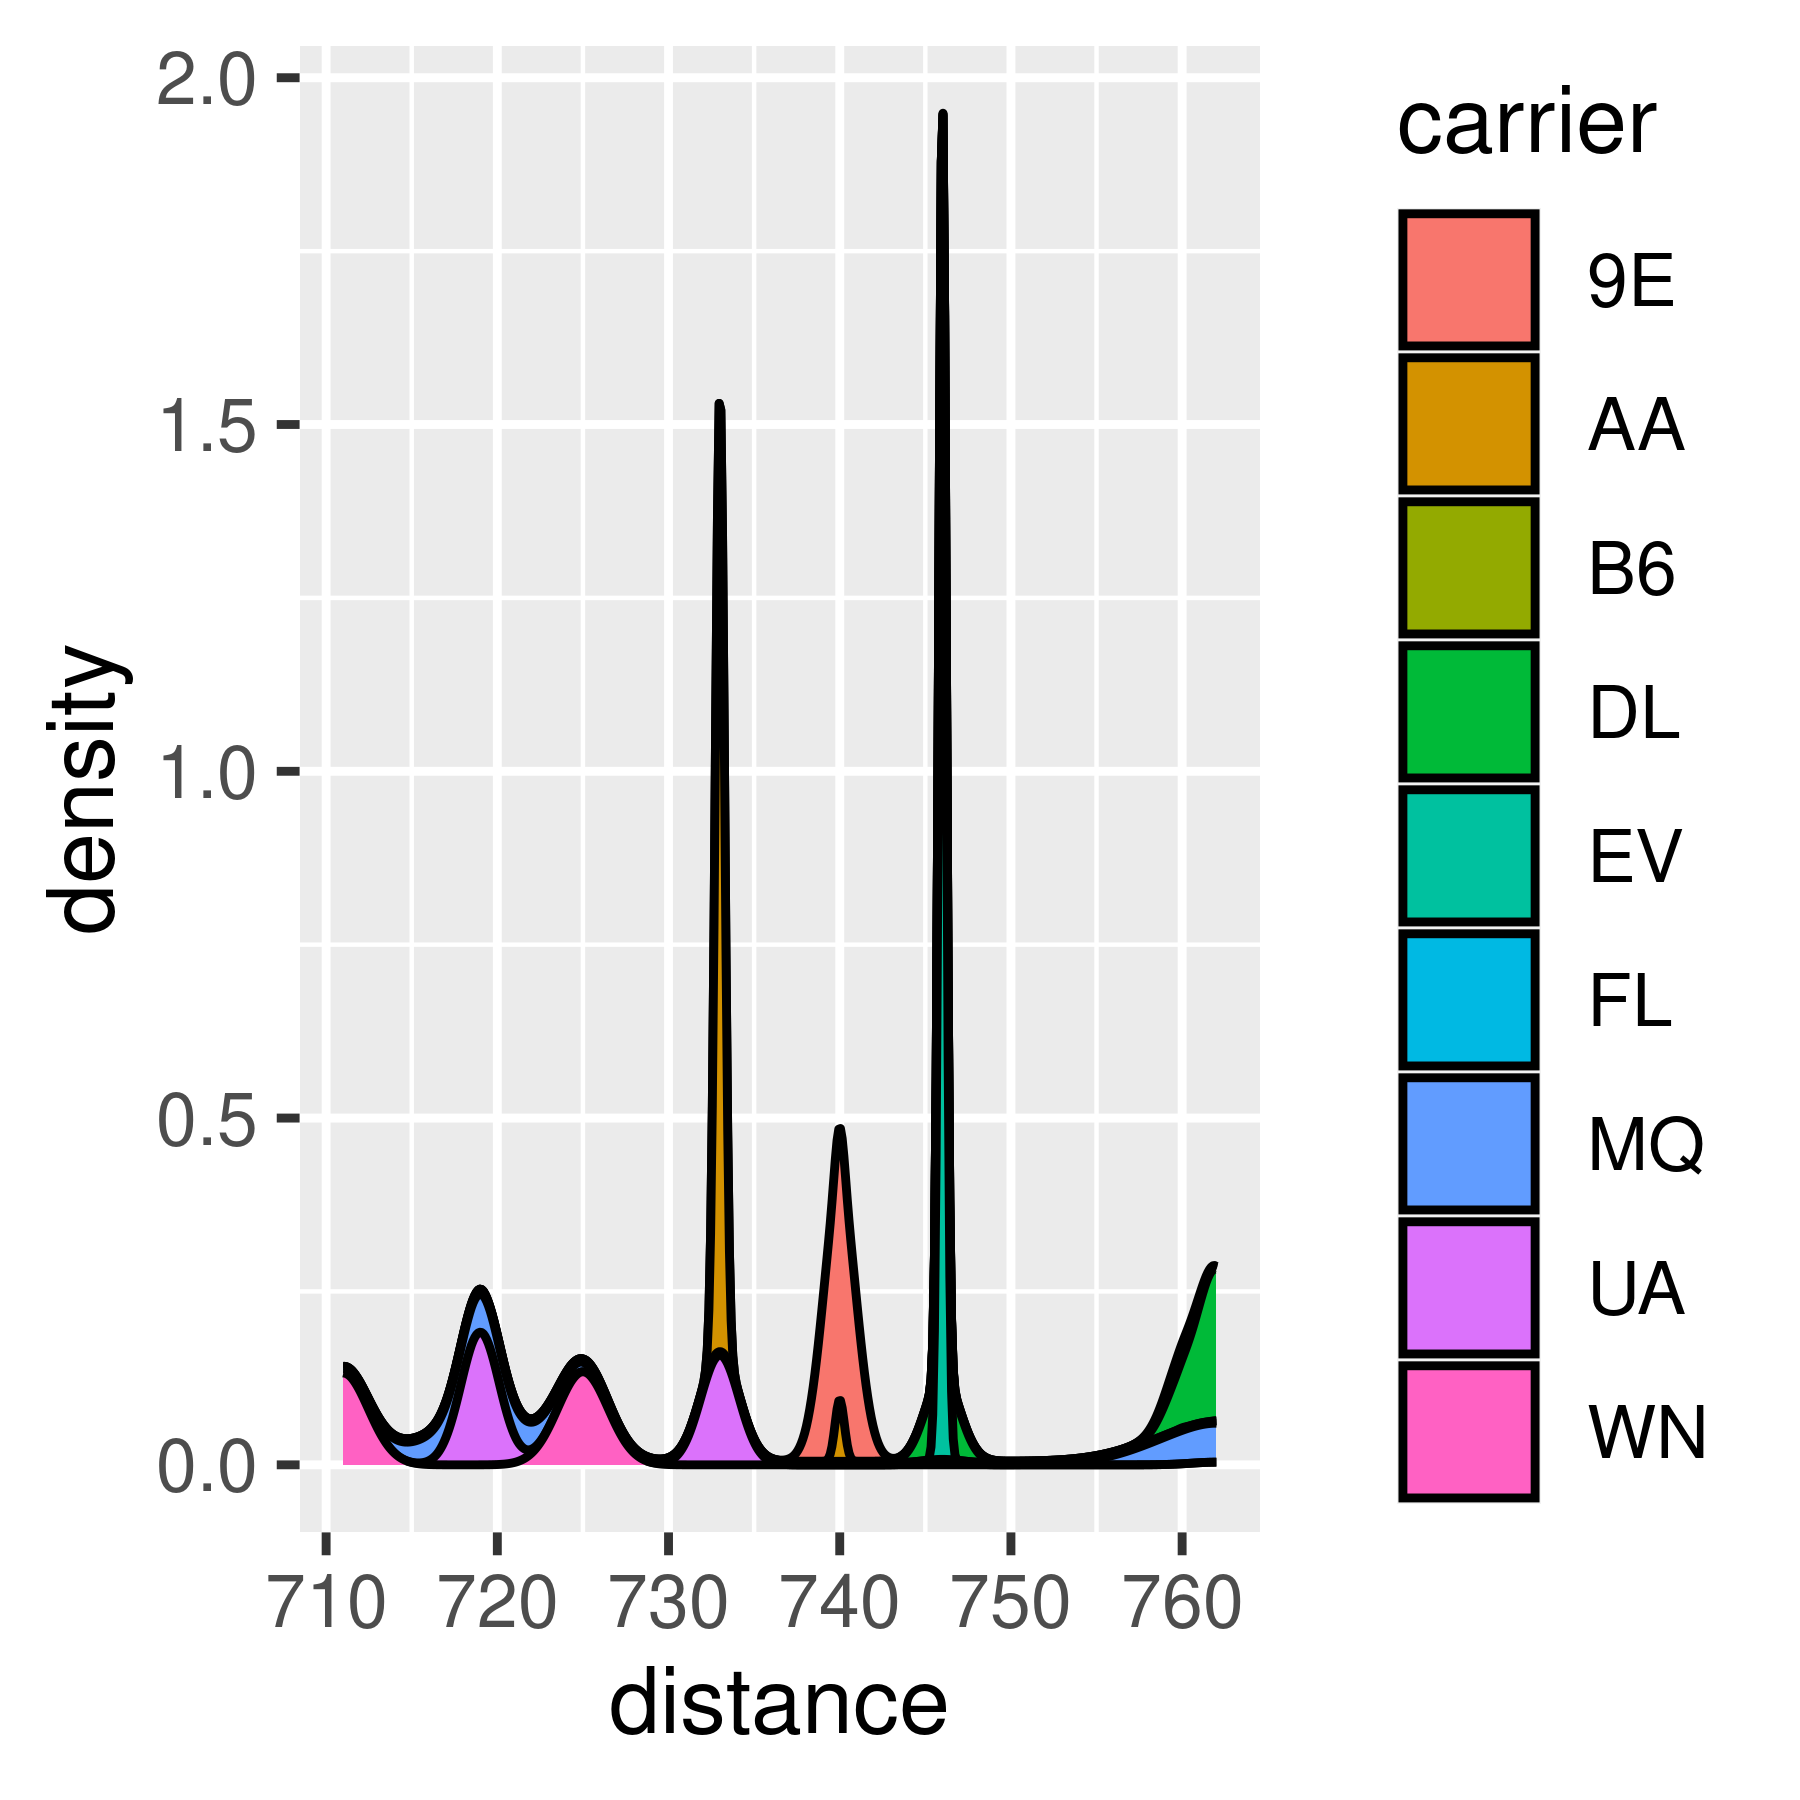
\includegraphics[width=.49\linewidth]{01-lit-review_files/figure-latex/flights_data_example-1} 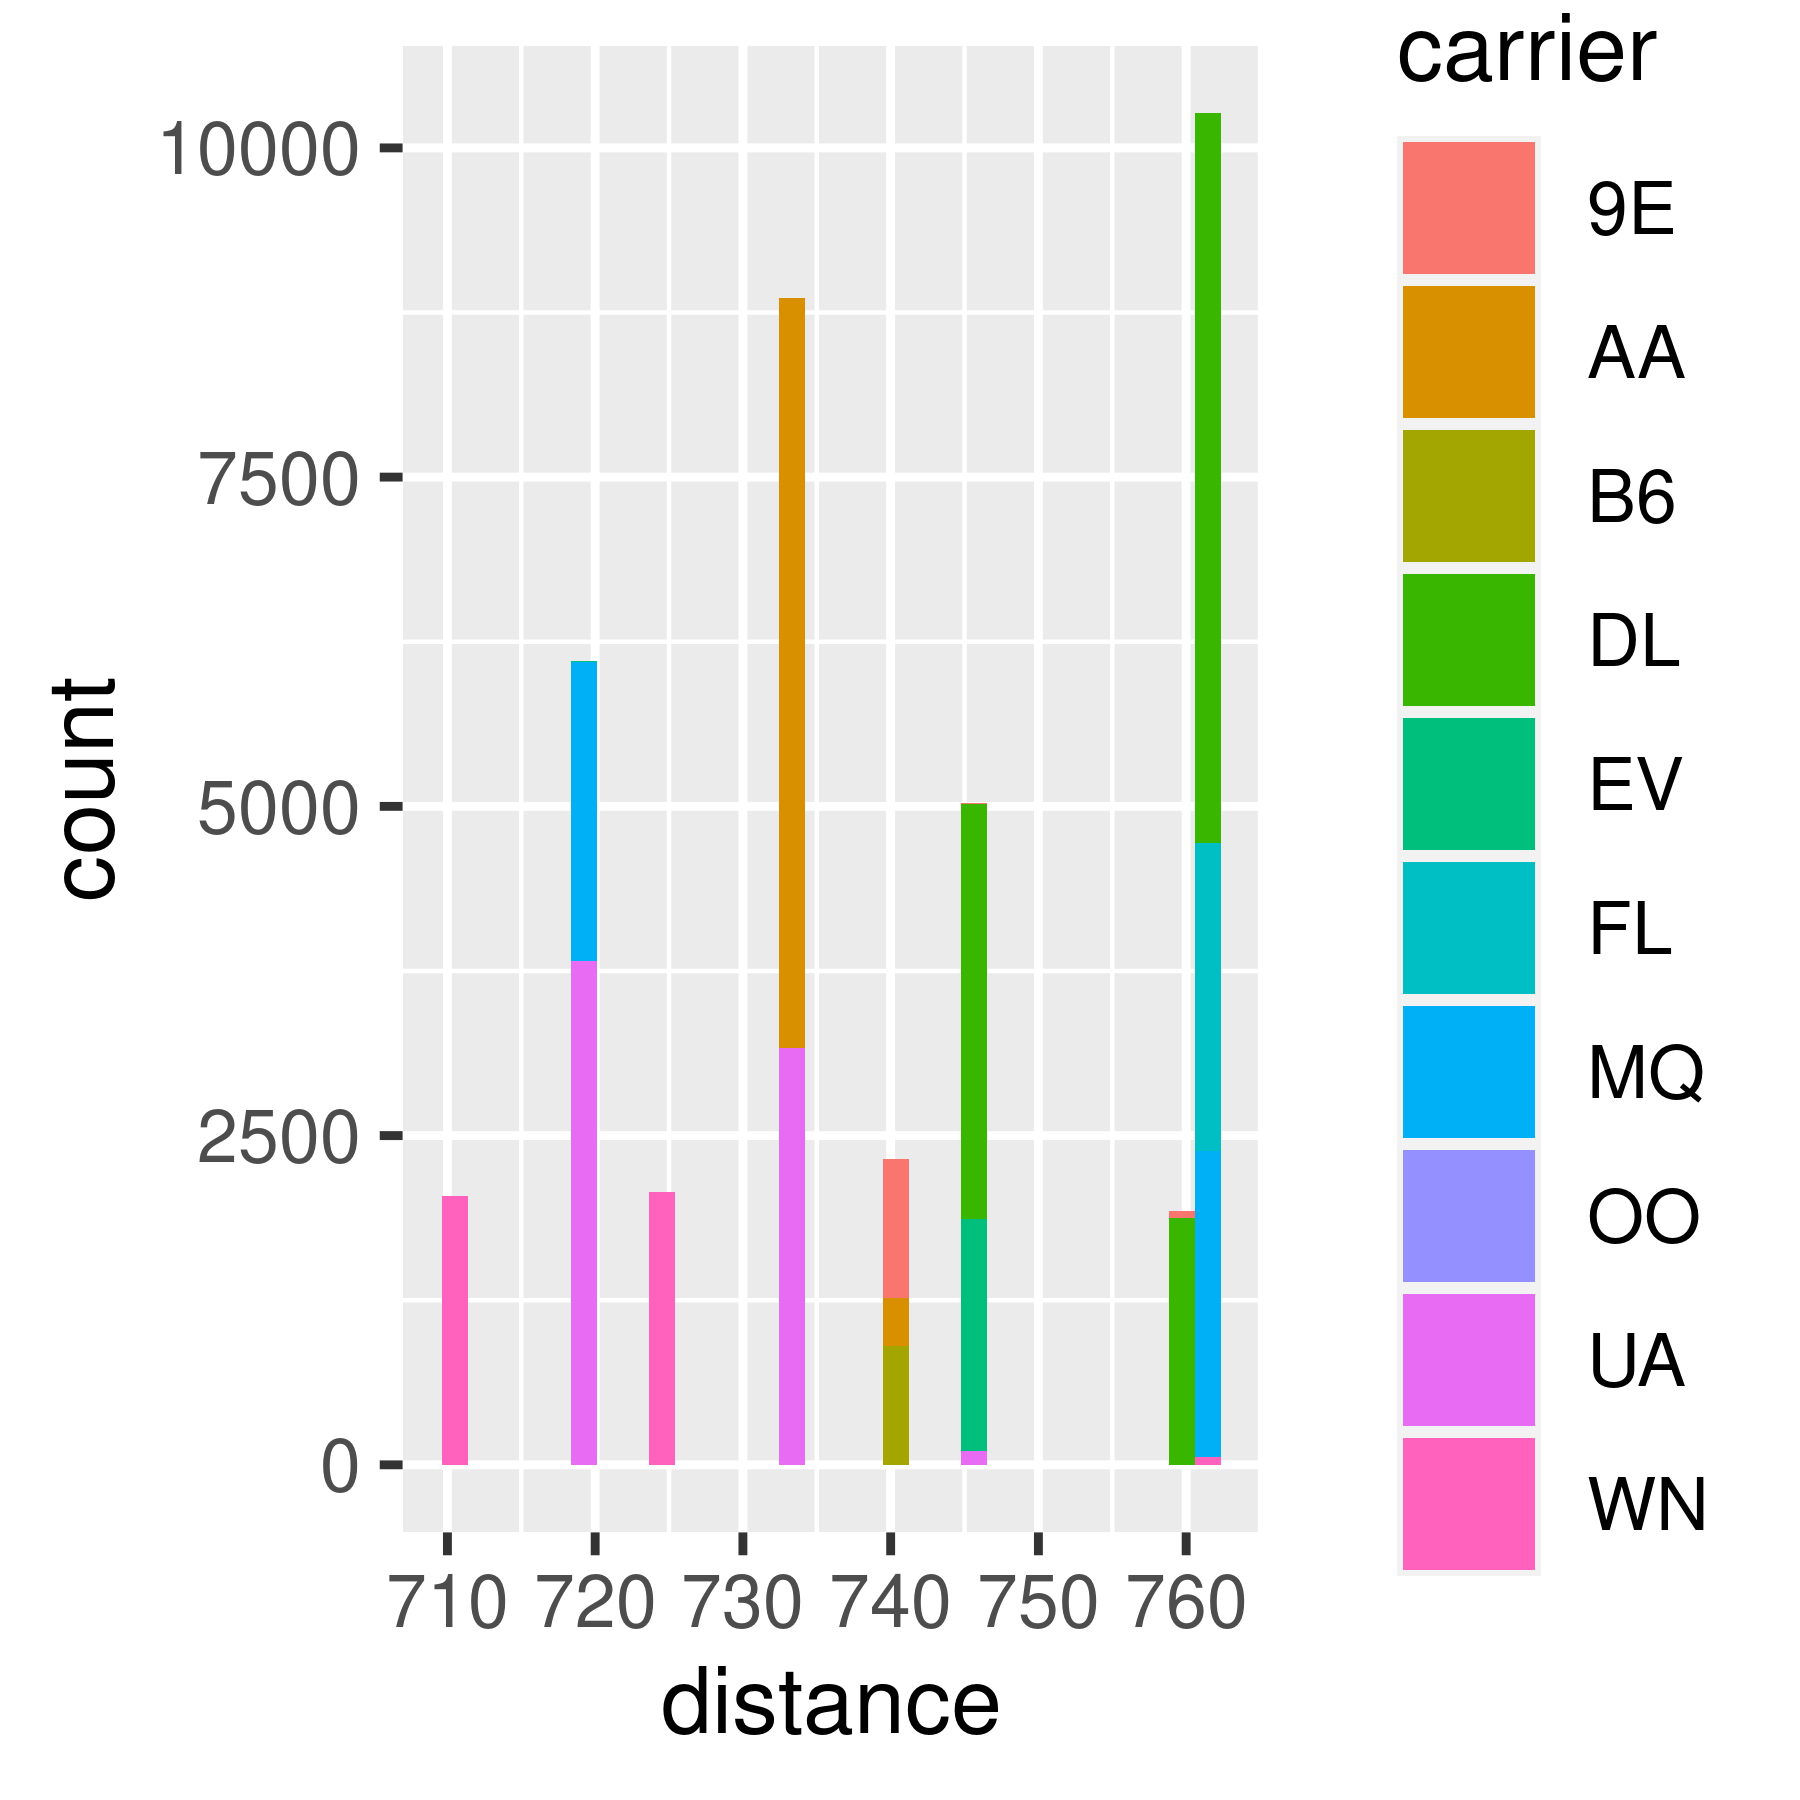
\includegraphics[width=.49\linewidth]{01-lit-review_files/figure-latex/flights_data_example-2} \end{center}

\db{On the other hand, Dashboards are interactive interfaces that display data visually to provide insights and support decision-making. 
Dashboards can be used to monitor key performance indicators, track progress over time, and identify patterns and trends in data. 
They often display real-time data and can be customized to show the most relevant data to the user.}

\db{Interactive graphics, are central to EDA [@unwin1999]. 
Beyond the limitations of static statistical displays, interactive graphics enable visualizations to advance alongside the analysis. 
User interaction and direct manipulation are required for dynamic graphics to reach their full potential (@cook1995; @unwin1999).
The connection between EDA and dashboards is that EDA is the process of preparing and understanding the data, which is the first step for building a dashboard, as the data has to be cleaned, transformed, and analyzed to be used efficiently on the dashboard. 
EDA results can be used to identify the most relevant data and metrics to include in the dashboard and to design the visualizations that will be used to display the data. 
And also, the EDA process can be used to identify the outliers, patterns, trends, and insights that will be useful to show in the dashboard to support decision-making.}

\db{Visualizations of data are essential for exploratory data analysis (EDA) along with model diagnostics. 
Plots for EDA are a valuable tool for guiding an analyst in discovering the relationships between variables in their data. 
When using plots in model diagnostics, plots help analysts determine whether or not the model is an appropriate way to model. 
During the initial EDA stage, an analyst may find that a variable or a covariate is directly related to the dependent variable when looking at a correlation heatmap or a scatterplot. 
This will be important to know before starting a linear model analysis. 
Much of our general understanding is from introductory statistics courses. 
The basic understanding can be formalized to visualize the discovery process.}

\hypertarget{variable-types}{%
\subsubsection{Variable Types}\label{variable-types}}

Not all variables should be used to create all types of charts -
variable type informs chart structure \db{
Categorical Data Visualization is the process of visualizing data that can be divided into distinct categories or groups. Categorical data are non-numeric and often represented by words, labels, or symbols, such as gender, product type, color, etc.}

\db{Visualizing categorical data helps uncover patterns and relationships between categories and can provide insights into the data distribution. 
Categorical data visualization techniques include bar charts, pie charts, histograms, stacked bar charts, and others. 
The choice of visual representation will depend on the data's nature and the insights being sought. 
The goal of categorical data visualization is to communicate the information effectively and make it easier to understand and interpret.}

\db{Friendly detailed using SAS with hands-on experiments to present categorical data analysis visually [@friendly2014]. 
Researchers have used PCPs to visualize categorical data. 
Beygelzimer, Perng, Ma and Hellerstien created a fast ordering categorical data analysis algorithm that helped visualization, where their algorithms helped organize the original parallel coordinate plots clearer ([@beygelzimer2001]; [@ma2001]). 
Hammock plots are modified versions of similar coordinate plots invented by Schonlau to visualize categorical data [@schonlau2003]. 
His design replaces coordinate polygons with rectangles to present the number. 
Treemaps are modified to support categorical data visualization.}

\db{CatTree gives a hierarchical categorical data visualization with interaction [@kolatch2001]. 
Fernstad developed an interactive system combining parallel coordinates, tables, and scatterplot matrices for an overview explorative analysis. 
Thoroughly research categorical data visualization to support algorithm understanding. 
The novel contingency wheel presented by [@alsallakh2011] supports visual analytics in categorical data, and he measured association based on Pearson's residuals and used visual abstraction based on elements frequency.  }

\db{High-Dimensional Data Visualization represents complex data sets with many variables or features (also known as high-dimensional data). 
The goal is to find effective ways to express such data in a form that allows easy understanding, analysis, and interpretation.
This is typically achieved by reducing the dimensionality of the data, for example, by projecting the data onto a lower-dimensional space or by aggregating the data in some way. 
The resulting visualizations can then reveal patterns, relationships, and other insights that would otherwise be difficult to detect from the raw data. 
For example, high-dimensional data visualization techniques include scatter plots, parallel coordinate plots, heat maps, and many others.}

\db{A popular research area in visualization since high-dimensional data is always fuzzy to mining. 
Direct visualization includes geometric visualizations:}

\begin{itemize}
\tightlist
\item
  scatterplots: use dots in coordinate to present data points.
\item
  parallel coordinates: present each dimension as axes, and every data
  item intersects dimensions as a polygon line at a particular position
\item
  RadViz/ PolyViz
\item
  GridViz
\end{itemize}

\db{Besides these traditional geometric visualization methods, iconographic displays like human faces and star glyphs used funny ways to present multivariate data. 
Hierarchical methods are used widely in parallel coordinates, which give analysts an intuitive view of clustering information [@fua1999]; [@johansson2005]. 
Rearrange the dimensions by dimension similarity on parallel coordinates, circle segments, and recursive patterns [@ankerst1998]. 
Guo used an interactive feature selection method to help users identify interesting subspaces from high-dimensional data sets [@guo2003].}

\hypertarget{grammar-of-graphics}{%
\subsubsection{Grammar of Graphics}\label{grammar-of-graphics}}

\db{Frame as a way to easily change between appropriate forms of presentation for a given variable or set of variables.}

It doesn't help us decide which is better - for that we need user
testing.

\db{The grammar of graphics (gg of ggplot2) is a theory that is well-defined for creating statistical graphics with work from Wilkinson [@Wilkinson1999] and Hadley Wickham [@ggplot2]. 
The Grammar of Graphics is a framework for understanding the structure of statistical graphics developed by Leland Wilkinson. 
It proposes that any statistical graphic can be broken down into a set of essential components, or "grammar," that can be combined in different ways to create a wide range of visualizations. }

\db{Grammar of graphics is defined as the framework which follows a layered approach to describe and construct visualizations or graphics in a structured manner.}

The components of the grammar of graphics include:

\begin{itemize}
\tightlist
\item
  Data: The raw data being visualized represents a set of observations
  or values.
\item
  Aesthetic Mappings: The mapping of data variables to visual properties
  such as position, color, shape, and size.
\item
  Scales: The mapping of data values to visual values, such as mapping a
  numerical value to a bar height.
\item
  Geometries: The basic shapes representing the data, such as points,
  lines, bars, and histograms.
\item
  Facets: The plot division into multiple subplots, each representing a
  different subset of the data.
\end{itemize}

\db{For example, a bar chart can be created by mapping a categorical variable to the x-axis, mapping a numerical variable to bar heights, and using rectangular bars as the geometry. 
For example, mapping two numerical variables can create a scatter plot to the x and y positions and use points as the geometry.
Finally, the Grammar of Graphics provides a systematic way of thinking about visualizations, making it easier to choose the appropriate visual representation for a given dataset.
}

\begin{figure}

{\centering 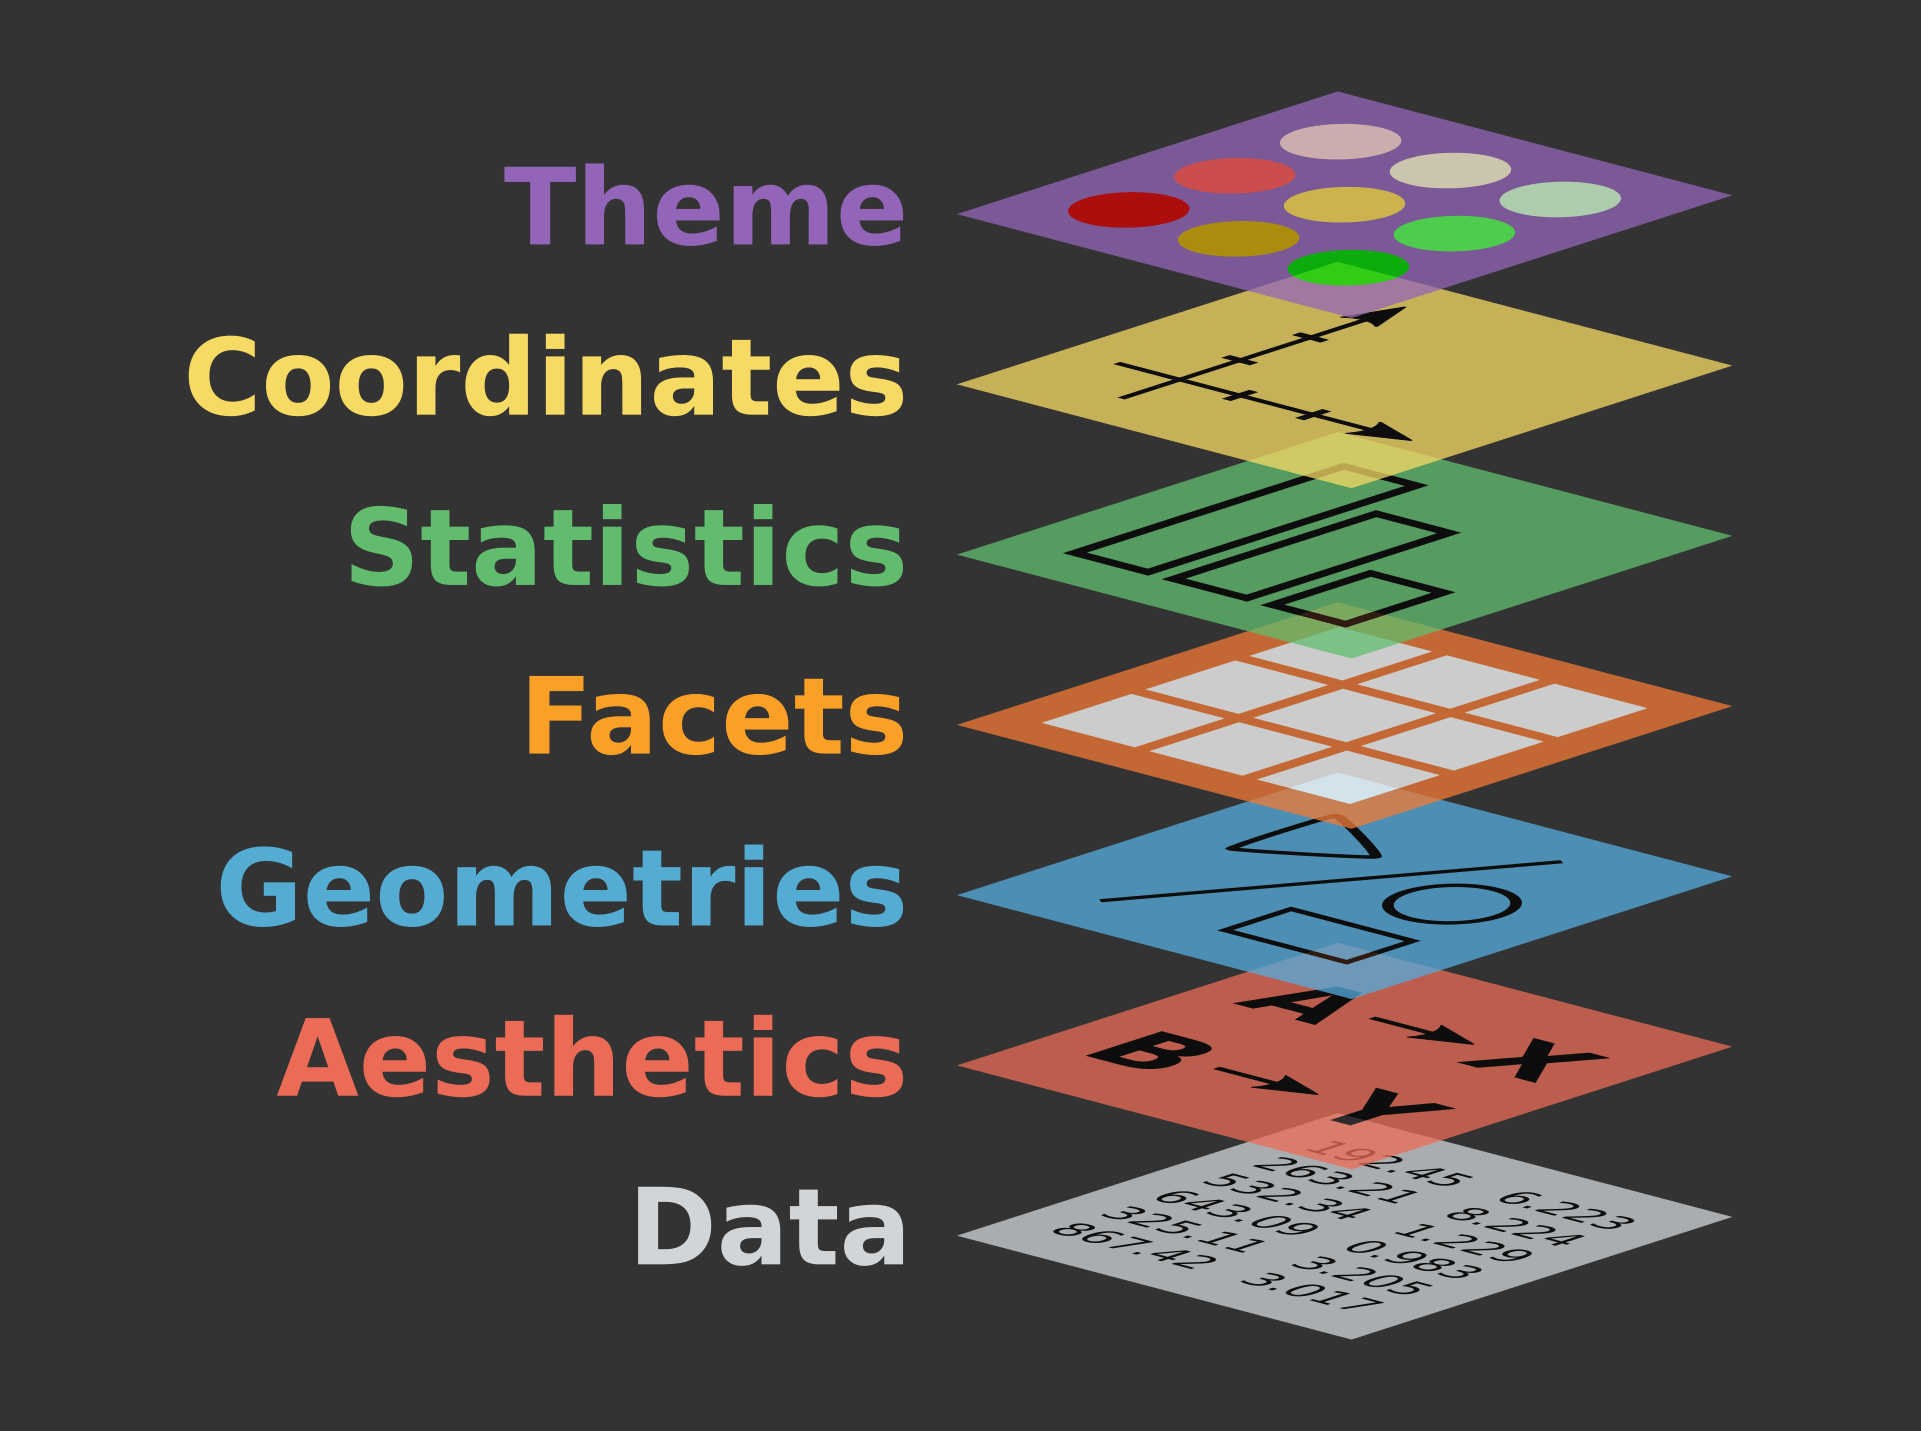
\includegraphics[width=0.45\linewidth]{figure/gglayers} 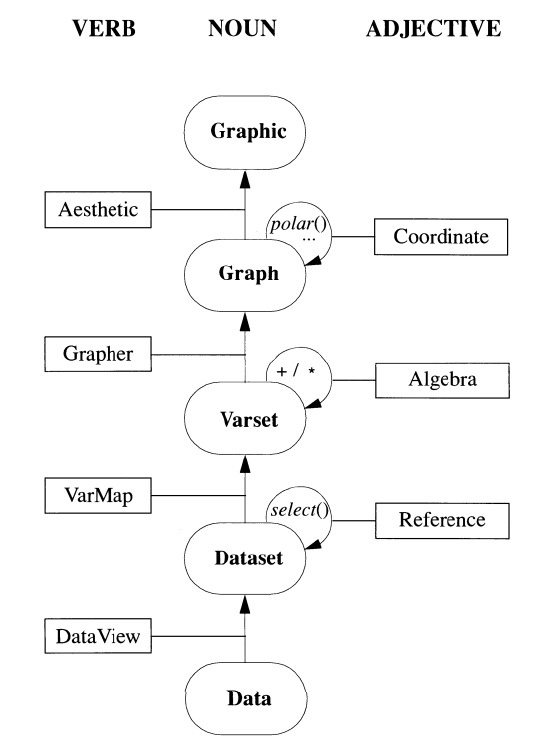
\includegraphics[width=0.45\linewidth]{figure/graphic-flowchart} 

}

\caption{Grammar of Graphics Diagram of Wickham and Wilkinson's work}\label{fig:graphics2}
\end{figure}

\hypertarget{interactive-graphics}{%
\paragraph{Interactive Graphics}\label{interactive-graphics}}

\db{The area of interactive graphics is still very much a work in progress despite existing as a field of research since the late 1960s—developments are driven partly by new technology, such as `d3` [@bostock2011]. 
Visualizations are more than just a picture. 
They are now a tool that facilitates analytic activity through different modes of interaction [@yi2007]. 
Visualization is context-free, as it can mean different things to different people depending on the situation [@parsons2014]. }

\db{The van Wijk Simple Visualization Model is a diagrammatic representation that provides a simple and effective way to understand and visualize the flow of information and data through a system. 
It is a commonly used tool in Exploratory Data Analysis (EDA), which is the initial step in the data analysis process. 
The van Wijk model can be used to represent the flow of data from data sources, through intermediate processing stages, to the final visualization of results. 
van Wiij's simple visualization model shows how insights are generated as the human participates in a feedback loop between reading and interacting with visualization [@van2005]. }

\db{This model is also context-free, allowing for the focus to be on the feedback loops between visualization and the user.}

\begin{center}
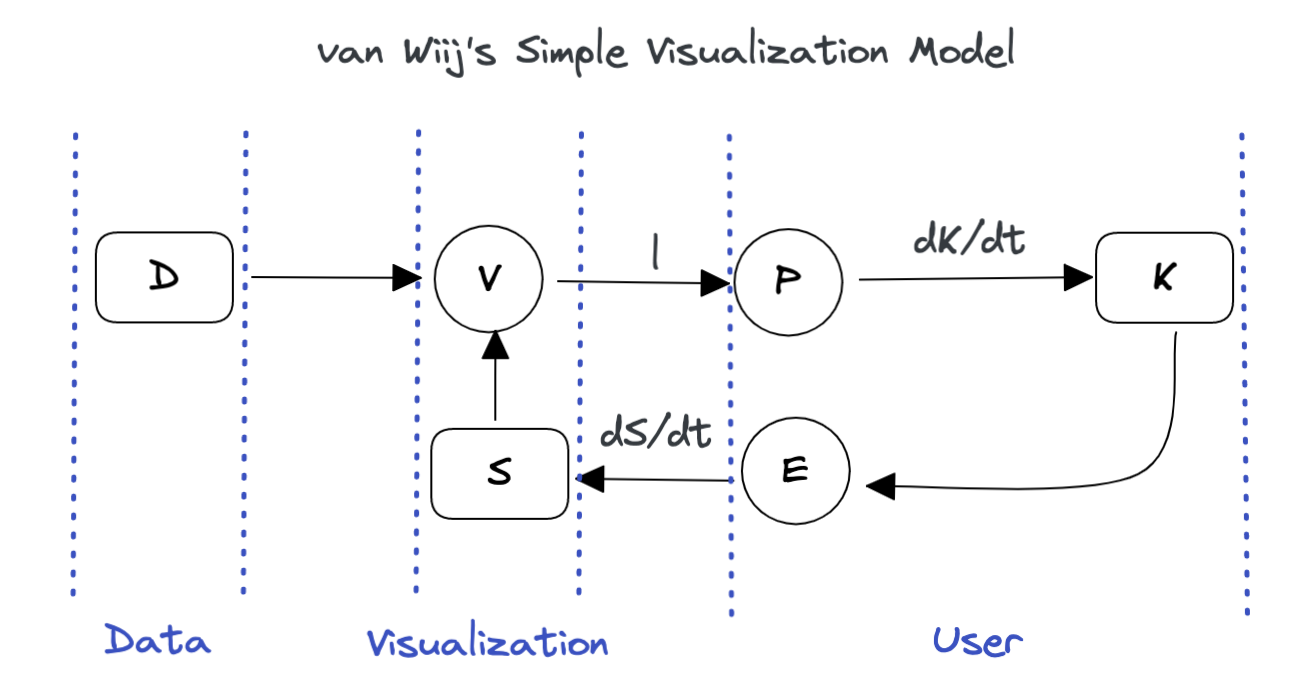
\includegraphics[width=\textwidth]{figure/vanWiijSimpleModel.png}
\captionof{figure}{van Wiij Simple Visualization Model}
\end{center}

\db{Interaction allows the user to define what data they see and how they see it, creating a dialogue between the user and the system. 
Theories behind visual representation include:}

\begin{itemize}
\tightlist
\item
  graphical comprehension ({[}@cleveland1984{]})
\item
  preattentive processing ({[}@ware2012{]})
\item
  gestalt theory ({[}@few2009{]})
\item
  graphical excellence ({[}@tufte2001{]})
\end{itemize}

Theories behind the manipulation of visualizations include but are not
limited to:

\begin{itemize}
\tightlist
\item
  cognitive fit ({[}@vessey1991{]})
\item
  visual perceptual approaches ({[}@baker2009{]})
\item
  human information processing
\end{itemize}

\db{As interactive visualizations play a more significant role in information systems, designers must know what tasks, visual representations, and interaction techniques are available and how they work to facilitate analytical reasoning. 
They must decide on the most effective visual representation without being able to estimate every user's ability to read and interpret the visualization.}

\db{Interactive visualization is a commonly used tool in Exploratory Data Analysis (EDA), which is the initial step in the data analysis process. 
The goal of EDA is to gain a high-level understanding of the data and to identify patterns, relationships, and anomalies in the data. }

\db{Visualizations have become more effective in recent years due to the pandemic and the Johns Hopkins University COVID-19 Dashboard [@JHPHDashboard] [Dashboard](https://coronavirus.jhu.edu/map.html).
We were glued to our computers, TVs, and phones for most of the world. 
As a result, we watched the dashboard change in real-time to adapt to the users' needs. 
In part to data growth and changing, the dashboard, as well as the visualizations, were needed in a condensed platform. 
The need to be concise and vastly informative is a struggle regarding data visualizations. }

\db{The human brain can only take in a set amount of data from a table or a paragraph. \svp{references?}
The space of infographics has been a much better way of looking at data on a creative scale.[@stat\_graph\_hist] 
While this may be a way of seeing the data in a friendly way, infographics need to include an interactive piece of data that many people would like to explore.}

\db{The relationship between the van Wijk Simple Visualization Model and Human-Computer Interaction (HCI) lies in the area of data visualization. 
The van Wijk Model provides a framework for understanding how information and data flow through a system to be displayed to the user. 
In the context of HCI, the model helps to understand how data is processed, transformed and presented to the user in a way that is intuitive, informative and engaging. 
The model helps to identify the various steps involved in the visualization process, from the collection and processing of data to the presentation of results. 
By doing so, it supports the design of more effective and user-friendly visualizations, which can enhance the overall user experience.}

\}

\hypertarget{multivariate-data-displays}{%
\subsubsection{Multivariate Data
Displays}\label{multivariate-data-displays}}

\begin{itemize}
\tightlist
\item
  Difficulty of visualizing multivariate data
\item
  Different approaches - briefly mention

  \begin{itemize}
  \tightlist
  \item
    encoding with shape/color/etc.
  \item
    tours
  \item
    pcps
  \item
    linked graphics (interactivity)
  \end{itemize}
\end{itemize}

This section doesn't need to solve the problem - it just introduces it

\hypertarget{audience-data-interactions}{%
\subsection{Audience-Data
Interactions}\label{audience-data-interactions}}

\db{User analysis is a crucial step in the design of user interfaces, especially in Human-Computer Interaction (HCI) and User Experience (UX) design. 
It involves studying the users of a system to understand their needs, goals, and behaviors. 
The purpose of user analysis is to create interfaces that are easy to use, efficient, and effective for the intended audience.}

Several methods can be used to conduct user analysis:

\begin{itemize}
\tightlist
\item
  Interviews: This involves conducting in-depth interviews with users to
  understand their needs, goals, and workflows.
\item
  Surveys involve sending out surveys to users to gather data on their
  needs and preferences.
\item
  Observations: This involves observing users as they complete tasks
  with the interface to understand their behaviors and workflows.
\item
  Personas: This is a method of creating fictional characters that
  represent the different types of users; it helps to understand the
  users' needs and goals.
\item
  Scenarios: This is a method of creating stories that describe how a
  user might interact with a system; it helps to understand the context
  and the user's needs.
\item
  Focus groups: This is a method of gathering a small group of users and
  facilitating a discussion to understand the users' needs and goals.
\item
  Contextual inquiry: This is a method of visiting the users in their
  work environment and observing them while they work; it helps to
  understand the context and the user's needs.
\end{itemize}

\db{The results of user analysis can be used to inform the design of the interface, including the layout, navigation, and functionality. 
It can also be used to identify areas of the interface that are confusing or difficult to use and to make recommendations for improvements. 
User analysis is an iterative process, and it should be done in multiple stages of the design process to ensure that the final product is tailored to the users' needs.}

\hypertarget{testing-static-graphics}{%
\subsubsection{Testing static graphics}\label{testing-static-graphics}}

Brief overview of user studies that compare different types of graphics,
accuracy, etc.

\db{Static Visualization is commonly used in the communication phase of data science workflows, and data scientists sometimes use them as part of the analysis. 
For example, John Tukey's EDA methods are currently known and well-vetted in the field. 
However, Satyanarayan et. al began to address this by introducing a high-level grammar of graphics called "Vega-Lite," which presents a set of standardized linguistic rules for producing interactive information visualizations using a concise JSON format for data to be represented by the grammar [@satyanarayan2016]. 
Vega-Lite has been directly implemented in R via the `ggvis` package using the same - albeit slightly lower-level.
Several protocols and methods can be used to test the design of a dashboard or other visual display. 
Some of these include:}

\begin{itemize}
\tightlist
\item
  Usability testing: This involves having users interact with the
  dashboard and providing feedback on its usability, including how easy
  it is to navigate, understand, and use.
\item
  Cognitive walkthrough: This involves having experts in human-computer
  interaction evaluate the dashboard, focusing on the cognitive
  processes required to use it effectively.
\item
  Eye-tracking: This involves using technology to track the users' gaze
  and interactions, to understand the user's focus and attention on the
  dashboard elements.
\item
  A/B testing: This involves creating two versions of the dashboard,
  each with slightly different design elements, and comparing the
  results to see which design is more effective.
\item
  Surveys: This involves asking users to complete a survey that measures
  their satisfaction and understanding of the dashboard and to provide
  feedback on improvements.
\item
  Heat maps: This involves using heat maps to track where users are
  clicking on the dashboard to identify which elements are being used
  the most and which are being ignored.
\item
  Card sorting: This is a method to understand the users' mental models
  and how they would like to organize and categorize the data; it is
  helpful to understand how to structure the dashboard navigation.
\end{itemize}

\db{These are just a few examples of the many protocols and methods that can be used to test the design of a dashboard. 
The selection of the appropriate way will depend on the specific goals of the testing and the resources available.}

\db{Remember that the user's feedback is crucial in the testing process; it will provide the necessary insight to improve the design and make it more efficient.}

\hypertarget{testing-interactive-graphics}{%
\subsubsection{Testing interactive
graphics}\label{testing-interactive-graphics}}

Overview of testing methods for interactive graphics - talk aloud,
measuring user engagement, etc.
\db{Testing interactive graphics using human perception principles in psychology involves considering various aspects of human perception and cognition to evaluate the effectiveness and user experience of the graphics. Here are some steps you can follow to test your interactive graphics:}

\db{Usability testing: Conduct a usability test to assess the ease of use and accessibility of the graphics. 
This includes testing for navigation, user control, and overall user experience.}

\db{Perception of visual elements: Evaluate how the visual elements in your graphics, such as color, contrast, size, and position, impact the perception of the information being presented.}

\db{Cognitive load: Assess the cognitive load on the user by evaluating how easily they can process and understand the information being presented. Factors such as complexity, amount of information, and type of information presented can impact cognitive load.}

\db{Attention allocation: Observe where the user's attention is directed while interacting with the graphics. This can help identify areas that may require improvement or modification to better engage the user's attention.}

\db{Memory retention: Evaluate the user's ability to retain and recall information presented in the graphics. This can help determine the effectiveness of the design in supporting memory retention.}

\db{User feedback: Obtain user feedback through surveys, interviews, or focus groups to gain insights into the user experience and identify areas for improvement.}

\db{It is important to keep in mind that human perception and cognition can vary greatly between individuals and can be influenced by a range of factors, such as age, culture, and personal experience. Testing with a representative sample of your target audience can help ensure that your interactive graphics are optimized for a wide range of users.}

\hypertarget{dashboard-design}{%
\subsection{Dashboard Design}\label{dashboard-design}}

Given that the audience has limitations, there are design constraints
around the data, and the ability of the audience to successfully use the
graphical displays of the data, what can we take from this body of
research that applies to more complicated sets of graphics?

How do we maintain user attention, desire to explore, and accurately
communicate the data through the medium of an interactive data
dashboard?

\db{A dashboard is a visual display of the essential information needed to achieve one or more objectives, consolidated and arranged on a single screen so the information can be monitored at a glance [@few]. 
Dashboards have particular characteristics:}

\begin{itemize}
\tightlist
\item
  Achieve specific objectives
\item
  Fits on a single computer screen
\item
  Information can be displayed in multiple mediums (web browser or
  mobile device)
\item
  Can be used to monitor information at a high level
\end{itemize}

\db{Dashboards can present various statistical data, such as financial performance, website traffic, or customer engagement metrics. 
They allow users to quickly and easily understand complex data sets using visual elements such as charts, graphs, and tables to display the information. 
Additionally, statistics can be used to analyze data presented on a dashboard, providing insights into trends and patterns that can inform decision-making.}

\db{While a dashboard can be handy, it may be worth describing that a poorly designed dashboard will not be used. 
A dashboard should be concise, clear, and intuitive when displaying components in combination with a customized list of requirements of users.}

\db{Much of the work done within statistical research and dashboard design involves collaboration with other researchers and users. 
While this may be the best for the growth of the discipline, one will find that working with collaborators with non-STEM backgrounds.
Dashboards can help understand and support many data types in essential business objectives. 
There are many different ways to label and utilize dashboards in different kinds.}

\db{Dashboards are cognitive tools that should be used to improve understanding of data, which should help people visually find relationships, trends, patterns, and outliers. 
Most importantly, dashboards should leverage people's visual cognitive capabilities.}

\db{EDA refers to methods and procedures for exploring the data space to learn about a data set. 
By analogy, exploratory modeling analysis (EMA) refers to methods and procedures for exploring the space of models which may be fit to a data set.}

\db{Interactive graphics are excellent for EDA; they are designed for exploring rather than presenting information (and more) and can be obtained by directly querying the graphic [@unwin2003].}

\begin{itemize}
\tightlist
\item
  PCPs enable the display of multi-dimensional data in two-dimensional
  space.
\item
  There must be some loss of information, but this can be partly
  counteracted by varying the order of the axes.
\item
  Interactivity is valuable for reordering the axes flexibly and fast.
\item
  Interaction is valuable for dealing with the dense mass of lines
  produced by large data sets.
\end{itemize}

\db{Being able to select subgroups of cases, highlight the chosen lines, and switch between different subgroups all assist in interpreting the otherwise intricate displays which arise.}

\db{Cowan suggested that the average person can only hold two to six pieces of information in their attention [@cowan2001]. 
People can develop detailed understandings of reality, which is infinitely complex.}

\db{Cognitive structures consist of mental models and their relationships ([@rumelhart1976], [@carley1992], [@jonassen1996]).
A schema is a mental model containing a breadth of information about a specific object or concept. 
Schemas are organized into semantic networks based on their relationships to other schemas [@wertheimer1938], [@rumelhart1976].
This arrangement helps the brain process its experiences instead of storing every sensory observation; the brain only needs to maintain its schemas, which are good summaries of all previous observations. 
Some "memories" may even be complete recreations built with a schema [@bartlett1932], [@klein2007]}

\db{Wixon introduce "contextual design" as a systems development method in which the researcher partners with the user at the user's place of work to "develop a shared understanding" of the user's activities, and they define contextual inquiry as the first part of the broader process [@cowan2001]. 
Contextual inquiry is the data collection step of the field research element of the contextual design method, and it emphasizes four essential principles:}

\begin{enumerate}
\def\labelenumi{\arabic{enumi}.}
\tightlist
\item
  The context of the activity being performed by the user
\item
  The partnership between the researcher and the participant
\item
  The spoken verification that the investigator's interpretation of the
  activity matches the user's
\item
  The focus of the study is central to the approach taken by the
  interviewer
\end{enumerate}

\db{Kandal conducted what might be considered a contextual interview study similar to ours in that they analyzed data scientists' self-reported work processes [@kandel2012]. 
They proposes three main archetypes that data scientists may be classed into the following:}

\begin{itemize}
\tightlist
\item
  Hackers: who build processes chaining together multiple programming
  languages of different types (analytical, scripting, and database
  languages) and use visualization in various environments.
\item
  Scripters: who perform most of their analysis in an analytical
  environment (e.g., R or Python) and execute the most complex
  statistical modeling of the types but who do not performstatements
  their ETL
\item
  Application Users: who performed most or all of their work in an
  application such as Excel or SPSS and, like scripters, relied on
  others (namely, their organizations' IT departments) for ETL.
\end{itemize}

\hypertarget{conclusion}{%
\subsection{Conclusion}\label{conclusion}}

\db{In this dissertation, I address this question of design for dashboards, as well as tools which can be used to support the display of multivariate data in an interactive context.
Chapter 1 presents a thorough review of the literature regarding graphical and human computer interaction/UI-UX methods. 
Chapter 2 will explore the process of designing dashboards for public use thorough parallel coordinate plots as a central component to data exploration to make decisions.
Chapter 3 focuses on graphical methods for multidimensional categorical variables and visualization methods have for growth.
We conclude with a Shiny application that facilitates a better understanding of the possible forms a parallel coordinate plots in exploratory data analysis can take by accommodating a through examination through variables and structural changes to the parallel coordinate plot with a click of a mouse.
Chapter 4 further explores multidimensional categorical data visualizations and develops an approach to using parallel coordinate plots to assess predictive model. 
We identify visual indicators for parameters in different models and extend the connection between parallel coordinate plots of binary tables and odds ratios to include logistic regression models with categorical variables.
}

\end{document}
